\documentclass[]{article}
\usepackage{lmodern}
\usepackage{amssymb,amsmath}
\usepackage{ifxetex,ifluatex}
\usepackage{fixltx2e} % provides \textsubscript
\ifnum 0\ifxetex 1\fi\ifluatex 1\fi=0 % if pdftex
  \usepackage[T1]{fontenc}
  \usepackage[utf8]{inputenc}
\else % if luatex or xelatex
  \ifxetex
    \usepackage{mathspec}
  \else
    \usepackage{fontspec}
  \fi
  \defaultfontfeatures{Ligatures=TeX,Scale=MatchLowercase}
\fi
% use upquote if available, for straight quotes in verbatim environments
\IfFileExists{upquote.sty}{\usepackage{upquote}}{}
% use microtype if available
\IfFileExists{microtype.sty}{%
\usepackage{microtype}
\UseMicrotypeSet[protrusion]{basicmath} % disable protrusion for tt fonts
}{}
\usepackage[margin=1in]{geometry}
\usepackage{hyperref}
\hypersetup{unicode=true,
            pdftitle={MAthesis},
            pdfborder={0 0 0},
            breaklinks=true}
\urlstyle{same}  % don't use monospace font for urls
\usepackage{natbib}
\bibliographystyle{plainnat}
\usepackage{longtable,booktabs}
\usepackage{graphicx,grffile}
\makeatletter
\def\maxwidth{\ifdim\Gin@nat@width>\linewidth\linewidth\else\Gin@nat@width\fi}
\def\maxheight{\ifdim\Gin@nat@height>\textheight\textheight\else\Gin@nat@height\fi}
\makeatother
% Scale images if necessary, so that they will not overflow the page
% margins by default, and it is still possible to overwrite the defaults
% using explicit options in \includegraphics[width, height, ...]{}
\setkeys{Gin}{width=\maxwidth,height=\maxheight,keepaspectratio}
\IfFileExists{parskip.sty}{%
\usepackage{parskip}
}{% else
\setlength{\parindent}{0pt}
\setlength{\parskip}{6pt plus 2pt minus 1pt}
}
\setlength{\emergencystretch}{3em}  % prevent overfull lines
\providecommand{\tightlist}{%
  \setlength{\itemsep}{0pt}\setlength{\parskip}{0pt}}
\setcounter{secnumdepth}{0}
% Redefines (sub)paragraphs to behave more like sections
\ifx\paragraph\undefined\else
\let\oldparagraph\paragraph
\renewcommand{\paragraph}[1]{\oldparagraph{#1}\mbox{}}
\fi
\ifx\subparagraph\undefined\else
\let\oldsubparagraph\subparagraph
\renewcommand{\subparagraph}[1]{\oldsubparagraph{#1}\mbox{}}
\fi

%%% Use protect on footnotes to avoid problems with footnotes in titles
\let\rmarkdownfootnote\footnote%
\def\footnote{\protect\rmarkdownfootnote}

%%% Change title format to be more compact
\usepackage{titling}

% Create subtitle command for use in maketitle
\newcommand{\subtitle}[1]{
  \posttitle{
    \begin{center}\large#1\end{center}
    }
}

\setlength{\droptitle}{-2em}
  \title{MAthesis}
  \pretitle{\vspace{\droptitle}\centering\huge}
  \posttitle{\par}
  \author{}
  \preauthor{}\postauthor{}
  \date{}
  \predate{}\postdate{}

\usepackage{setspace}
\doublespacing

\begin{document}
\maketitle

{
\setcounter{tocdepth}{2}
\tableofcontents
}
\section{Time Bins with sample sizes}\label{time-bins-with-sample-sizes}

\begin{longtable}[]{@{}llrrrr@{}}
\caption{Time bins with age range, epoch name, mean age and
corresponding sample sizes (on individual, species and genus
level)}\tabularnewline
\toprule
bin & EpochBins & MeanBins & nIndividuals & nSpecies &
nGenera\tabularnewline
\midrule
\endfirsthead
\toprule
bin & EpochBins & MeanBins & nIndividuals & nSpecies &
nGenera\tabularnewline
\midrule
\endhead
(0,0.0117{]} & Modern & 0.00585 & 252 & 64 & 18\tabularnewline
(0.0117,0.126{]} & Upper Pleistocene & 0.06885 & 47 & 16 &
8\tabularnewline
(0.126,0.781{]} & Middle Pleistocene & 0.45350 & 48 & 11 &
6\tabularnewline
(0.781,2.59{]} & Lower Pleistocene & 1.68450 & 73 & 27 &
11\tabularnewline
(2.59,3.6{]} & Upper Pliocene & 3.09400 & 23 & 15 & 9\tabularnewline
(3.6,5.33{]} & Lower Pliocene & 4.46600 & 29 & 17 & 8\tabularnewline
(5.33,11.6{]} & Upper Miocene & 8.47000 & 52 & 23 & 9\tabularnewline
(11.6,16{]} & Middle Miocene & 13.78900 & 38 & 17 & 11\tabularnewline
(16,23{]} & Lower Miocene & 19.50000 & 25 & 13 & 9\tabularnewline
(23,50{]} & Oligocene and Eocene & 36.51500 & 7 & 5 & 5\tabularnewline
\bottomrule
\end{longtable}

\begin{figure}[htbp]
\centering
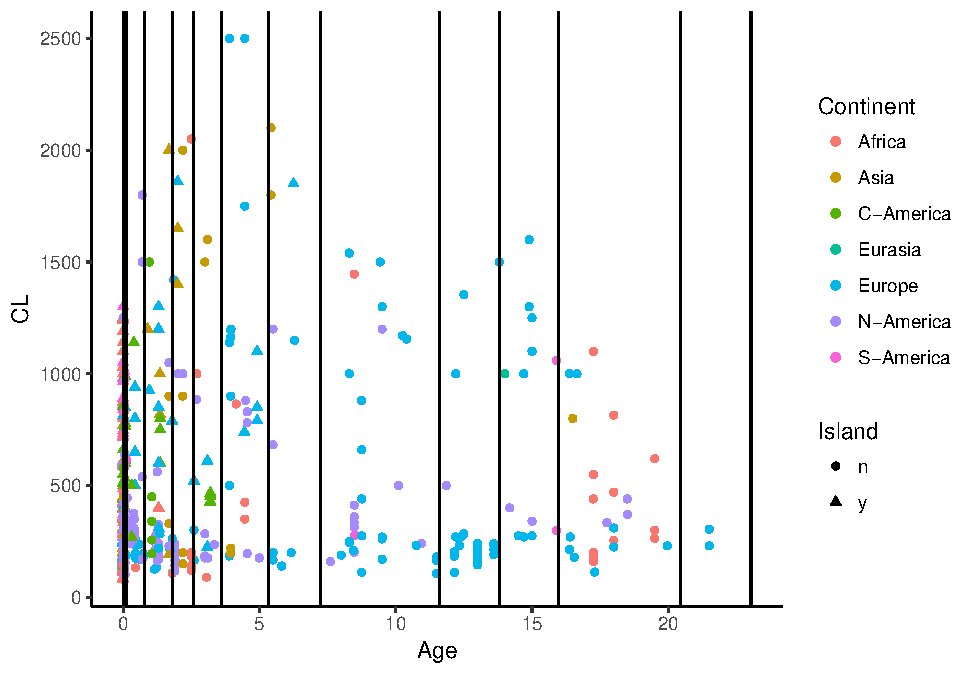
\includegraphics{MA_JJ_files/figure-latex/Get overview over data set-1.pdf}
\caption{Scatterplot of CL over time, indicating insular (triangle) and
continental (circles) and colour indicating continents.}
\end{figure}

\begin{verbatim}
## [1] 0
\end{verbatim}

\section{Smaller time bins}\label{smaller-time-bins}

\begin{longtable}[]{@{}llrrrr@{}}
\caption{Smaller time bins with age range, epoch name, mean age and
corresponding sample sizes (on individual, species and genus
level)}\tabularnewline
\toprule
bin & EpochBins & MeanBins & nIndividuals & nSpecies &
nGenera\tabularnewline
\midrule
\endfirsthead
\toprule
bin & EpochBins & MeanBins & nIndividuals & nSpecies &
nGenera\tabularnewline
\midrule
\endhead
(0,0.0117{]} & Modern & 0.00585 & 252 & 64 & 18\tabularnewline
(0.0117,0.126{]} & Upper Pleistocene & 0.06885 & 47 & 16 &
8\tabularnewline
(0.126,0.781{]} & Middle Pleistocene & 0.45350 & 48 & 11 &
6\tabularnewline
(0.781,1.81{]} & Lower Pleistocene & 1.29350 & 47 & 19 &
11\tabularnewline
(1.81,2.59{]} & Gelasian(LowPleio2) & 2.19700 & 26 & 10 &
7\tabularnewline
(2.59,3.6{]} & Upper Pliocene & 3.09400 & 23 & 15 & 9\tabularnewline
(3.6,4.47{]} & Lower Pliocene 1 & 4.02300 & 19 & 11 & 5\tabularnewline
(4.47,5.33{]} & Lower Pliocene 2 & 4.88900 & 10 & 7 & 4\tabularnewline
(5.33,7.42{]} & Upper Miocene 1 & 6.37800 & 12 & 9 & 6\tabularnewline
(7.42,9.52{]} & Upper Miocene 2 & 8.47000 & 30 & 13 & 7\tabularnewline
(9.52,11.6{]} & Upper Miocene 3 & 10.56200 & 10 & 7 & 5\tabularnewline
(11.6,13.8{]} & Middle Miocene 1 & 12.69850 & 22 & 8 & 6\tabularnewline
(13.8,16{]} & Middle Miocene 2 & 14.87950 & 16 & 13 & 10\tabularnewline
(16,18{]} & Lower Miocene 1 & 16.98500 & 19 & 10 & 8\tabularnewline
(18,23{]} & Lower Miocene 2 & 20.51500 & 6 & 4 & 4\tabularnewline
\bottomrule
\end{longtable}

\newpage

\section{Maps}\label{maps}

\subsection{fossil occurences of
testudinidae}\label{fossil-occurences-of-testudinidae}

\begin{figure}[htbp]
\centering
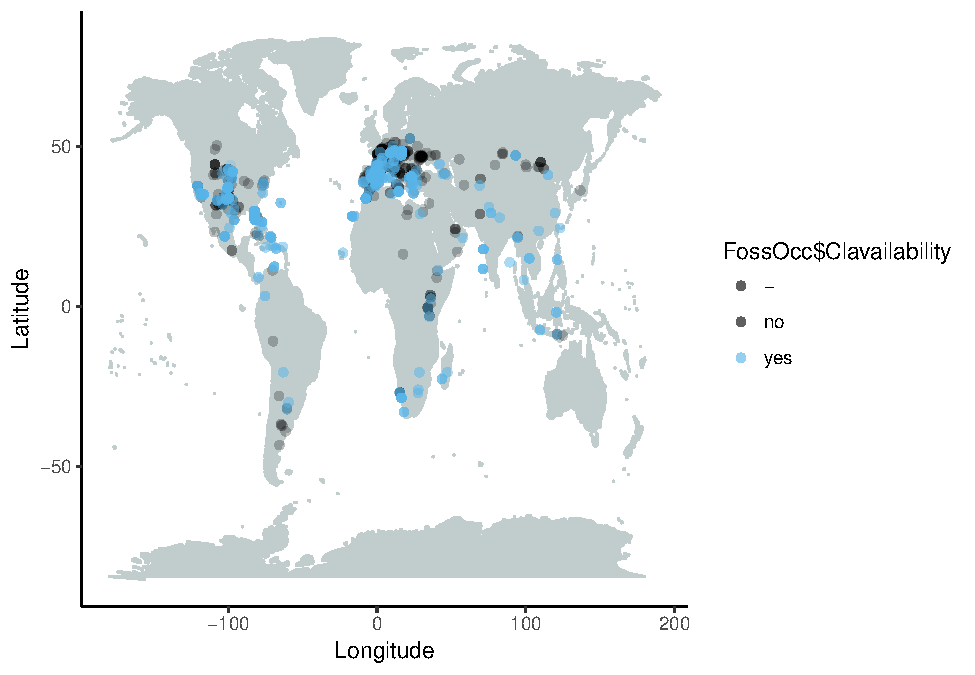
\includegraphics{MA_JJ_files/figure-latex/Map fossil occurrences-1.pdf}
\caption{Map displaying all fossil occurrences of testudinids, with
color indicating whether relevant literature was available (black if
not) and if it was, whether body size data was available or not (yes and
no, respectively).}
\end{figure}

\newpage

\subsection{body size of testudinidae}\label{body-size-of-testudinidae}

\begin{figure}[htbp]
\centering
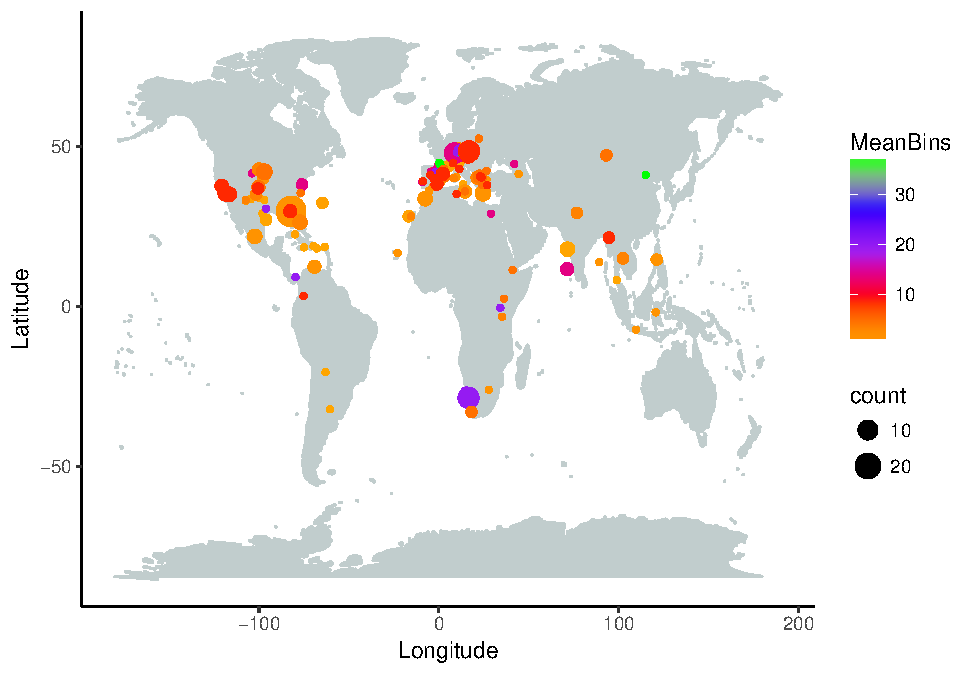
\includegraphics{MA_JJ_files/figure-latex/Map body size data set-1.pdf}
\caption{Map displaying all localities for which body size data for
testudinids was available in the literature. Size of points denotes
sample size, color denotes approximate age.}
\end{figure}

\newpage

\section{Sampling Accumulation Curve}\label{sampling-accumulation-curve}

\begin{figure}[htbp]
\centering
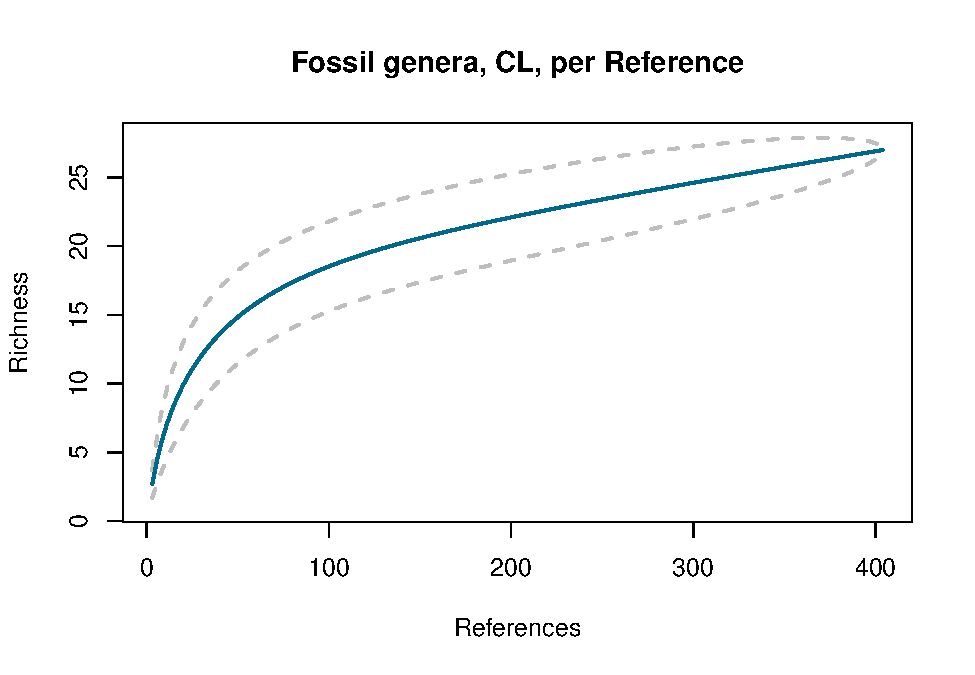
\includegraphics{MA_JJ_files/figure-latex/Species Accumulation Curve with Genera-1.pdf}
\caption{Sampling Accumulation Curve of fossil genera per reference}
\end{figure}

\subsection{Eurasia}\label{eurasia}

\begin{figure}[htbp]
\centering
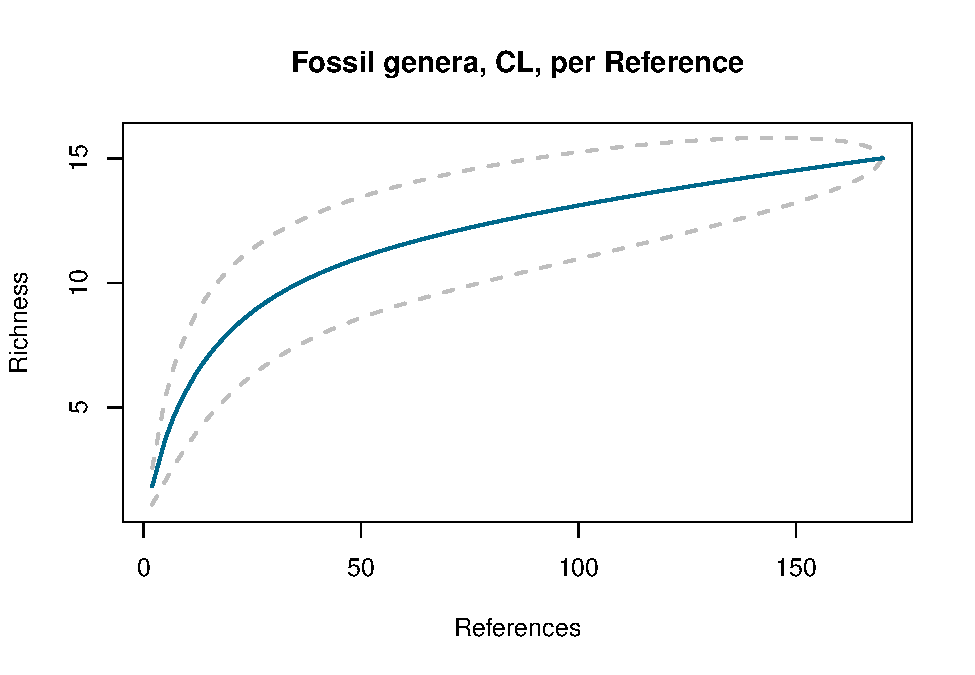
\includegraphics{MA_JJ_files/figure-latex/Species Accumulation Curve with Genera, Eurasia-1.pdf}
\caption{Sampling Accumulation Curve of fossil genera per reference,
Eurasia}
\end{figure}

\newpage

\section{Histograms}\label{histograms}

\subsection{all}\label{all}

\begin{verbatim}
## `stat_bin()` using `bins = 30`. Pick better value with `binwidth`.
\end{verbatim}

\begin{figure}[htbp]
\centering
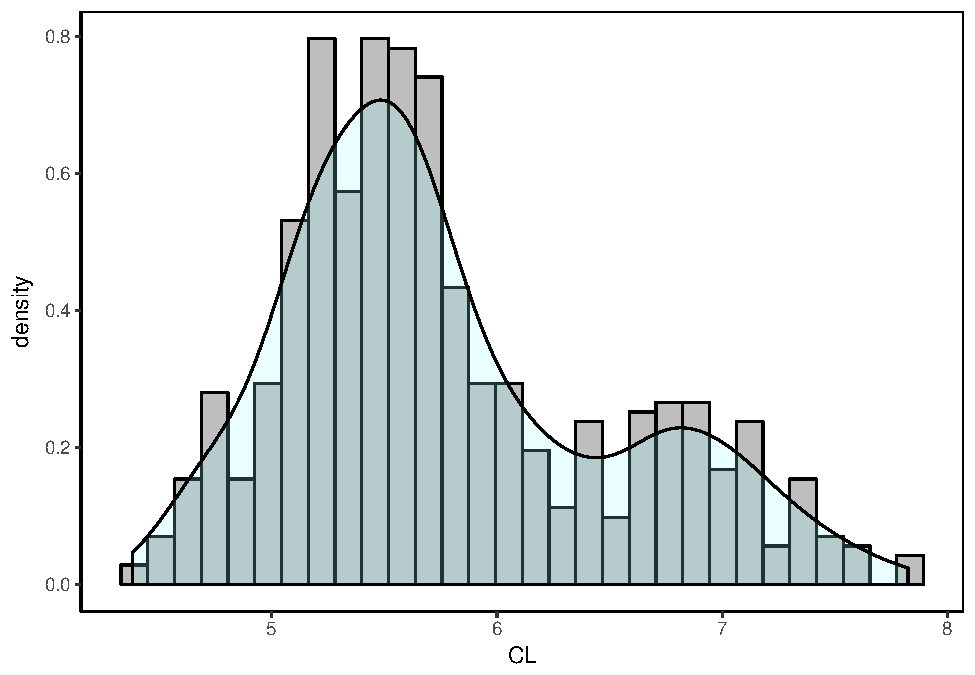
\includegraphics{MA_JJ_files/figure-latex/Histograms of body size data, all-1.pdf}
\caption{Distribution of body size data, logtransformed, all data.}
\end{figure}

\newpage

\subsection{per time bin}\label{per-time-bin}

\begin{verbatim}
## `stat_bin()` using `bins = 30`. Pick better value with `binwidth`.
\end{verbatim}

\begin{figure}[htbp]
\centering
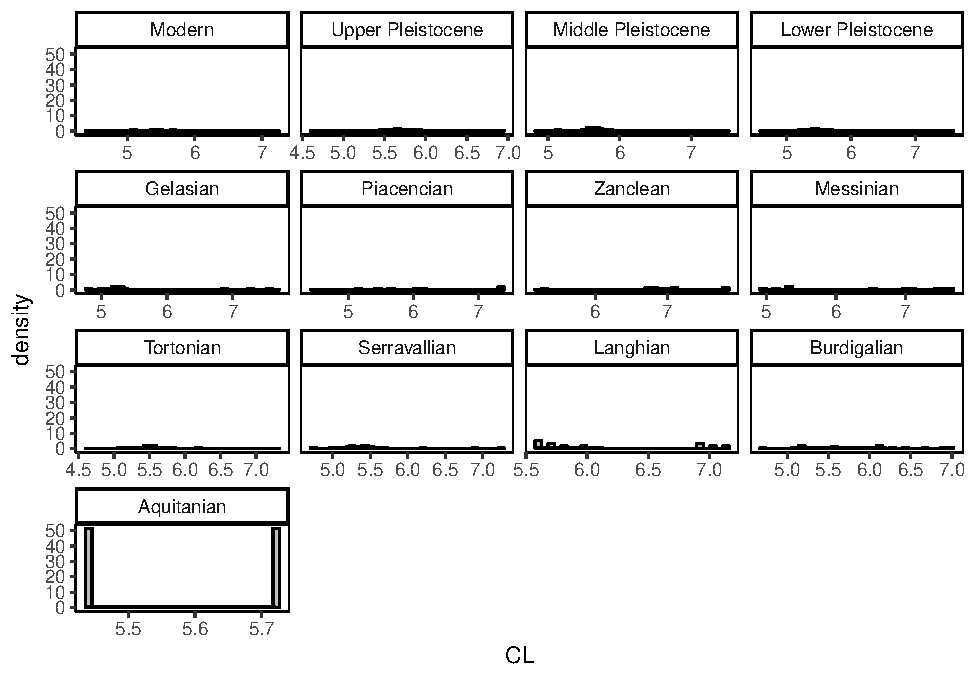
\includegraphics{MA_JJ_files/figure-latex/Histograms of body size data, per time bin-1.pdf}
\caption{Distribution of body size data per time bin, logtransformed.}
\end{figure}

\newpage

\subsection{modern vs.~fossil}\label{modern-vs.fossil}

\begin{verbatim}
## `stat_bin()` using `bins = 30`. Pick better value with `binwidth`.
\end{verbatim}

\begin{figure}[htbp]
\centering
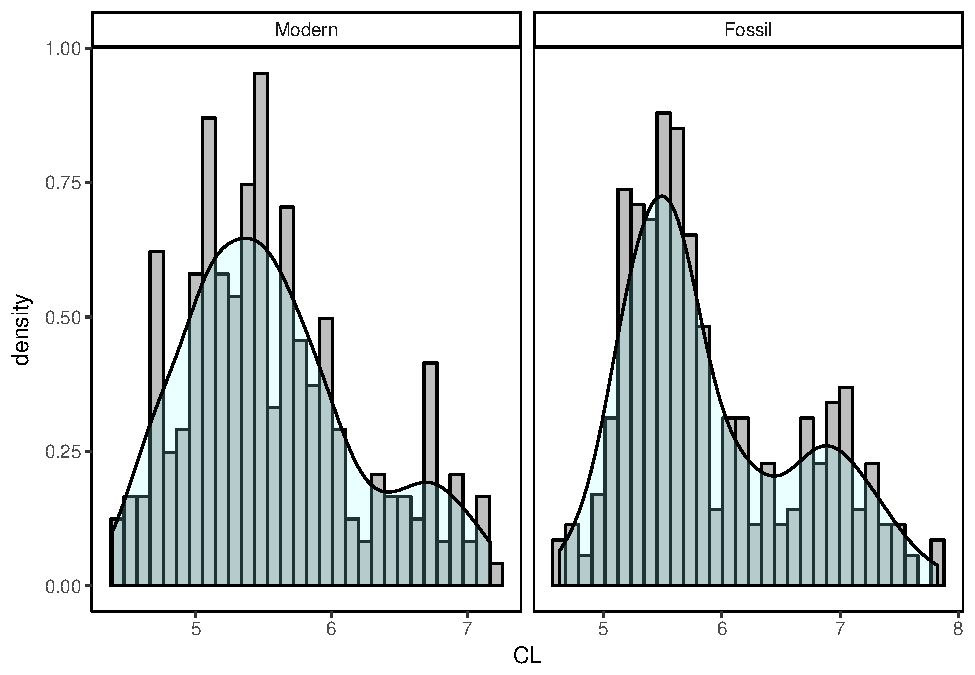
\includegraphics{MA_JJ_files/figure-latex/Histograms of body size data, modern vs. fossil-1.pdf}
\caption{Distribution of body size data modern vs.~fossil,
logtransformed.}
\end{figure}

\newpage

\subsection{modern vs.~fossil, continental
vs.~insular}\label{modern-vs.fossil-continental-vs.insular}

\begin{verbatim}
## `stat_bin()` using `bins = 30`. Pick better value with `binwidth`.
\end{verbatim}

\begin{figure}[htbp]
\centering
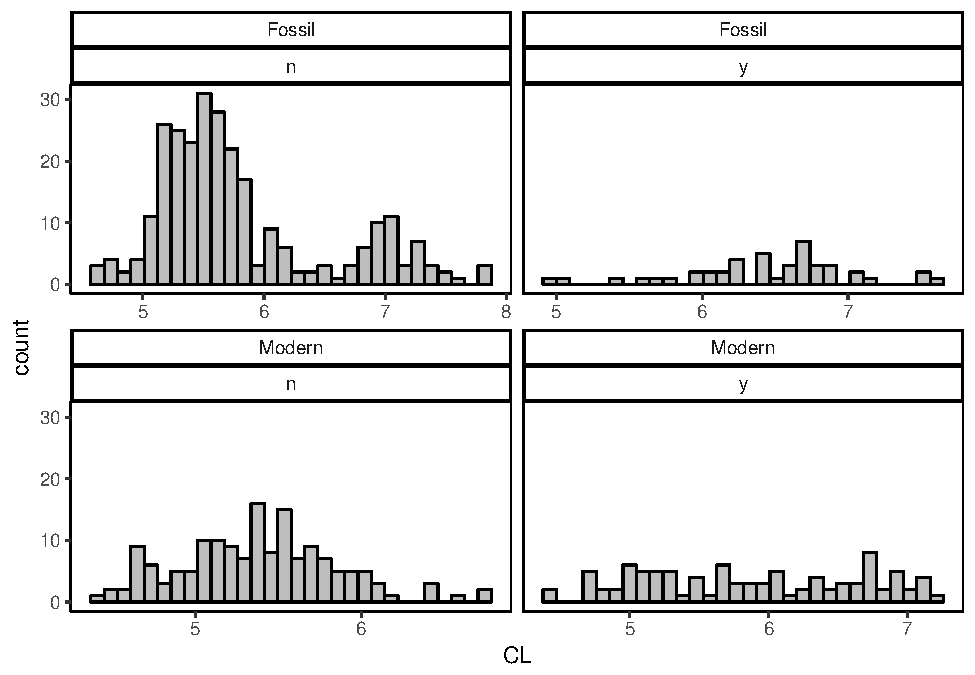
\includegraphics{MA_JJ_files/figure-latex/Histograms of body size data, modern vs. fossil, continental vs. insular-1.pdf}
\caption{Distribution of body size data modern vs.~fossil, continental
vs.~insular logtransformed.}
\end{figure}

\newpage

\subsection{continental vs.~insular}\label{continental-vs.insular}

\begin{verbatim}
## `stat_bin()` using `bins = 30`. Pick better value with `binwidth`.
\end{verbatim}

\begin{figure}[htbp]
\centering
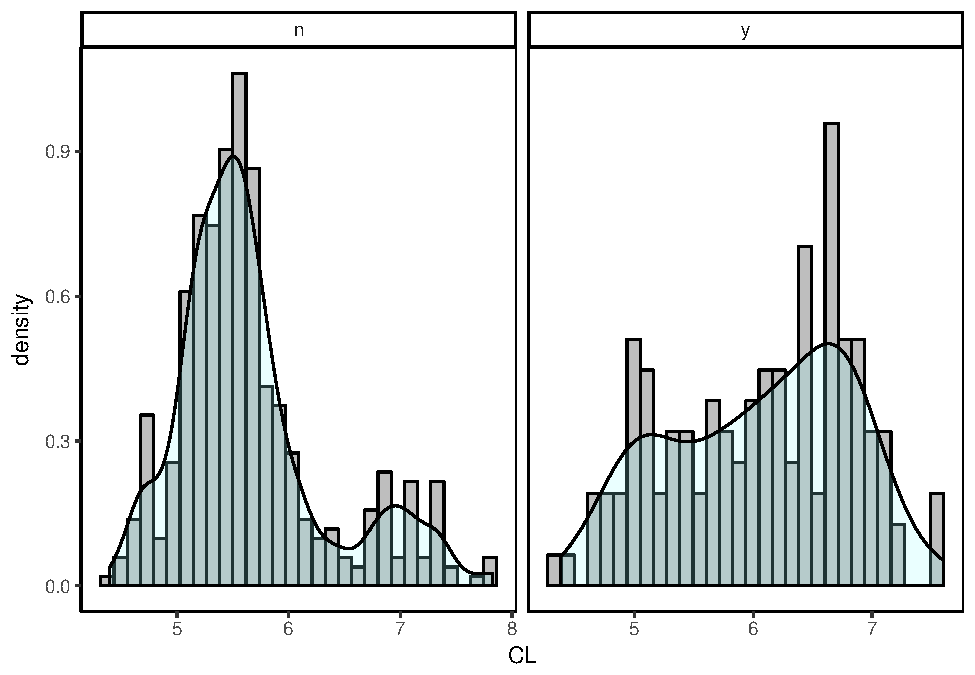
\includegraphics{MA_JJ_files/figure-latex/Histograms of body size data, continental vs. insular-1.pdf}
\caption{Distribution of body site data of continental (n) and
insular(y) species, logtransformed.}
\end{figure}

\newpage

\subsection{continents}\label{continents}

\begin{verbatim}
## `stat_bin()` using `bins = 30`. Pick better value with `binwidth`.
\end{verbatim}

\begin{figure}[htbp]
\centering
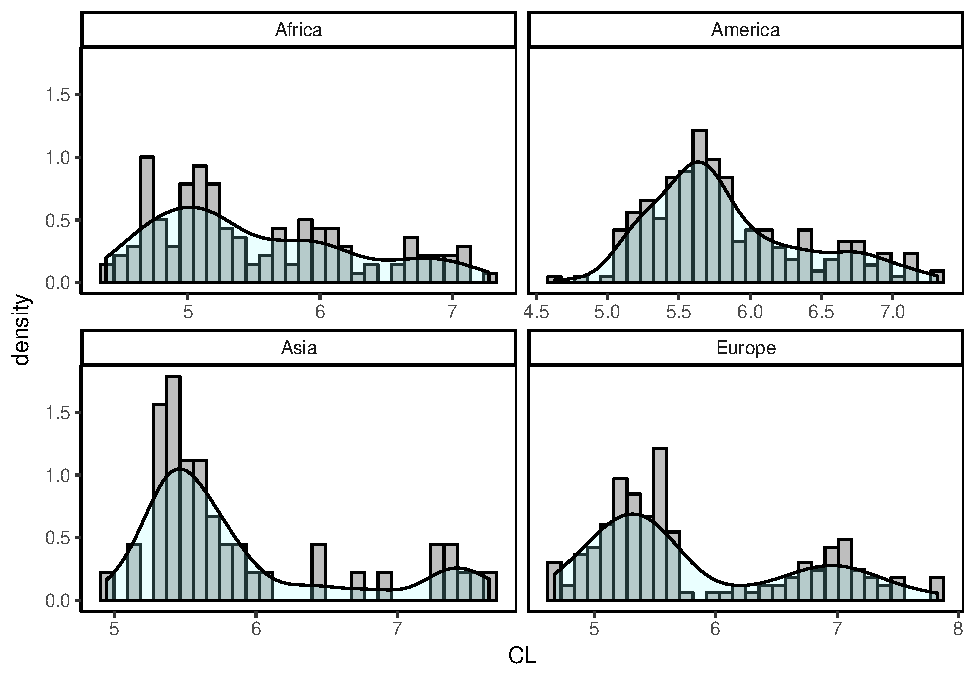
\includegraphics{MA_JJ_files/figure-latex/Histograms of body size data, split by continents-1.pdf}
\caption{Distribution of body site data per continent, logtransformed.}
\end{figure}

\newpage

\subsection{Genera}\label{genera}

\begin{verbatim}
## `stat_bin()` using `bins = 30`. Pick better value with `binwidth`.
\end{verbatim}

\begin{figure}[htbp]
\centering
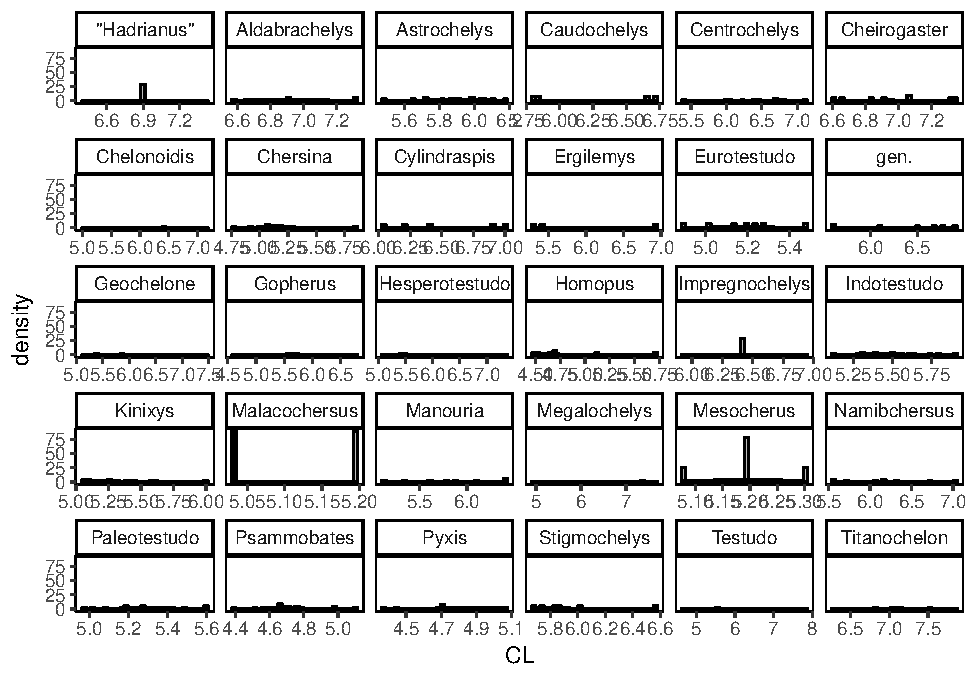
\includegraphics{MA_JJ_files/figure-latex/Histograms of body size data, genera-1.pdf}
\caption{Distribution of body size, genera, logtransformed.}
\end{figure}

\begin{longtable}[]{@{}lrrrrrrrrrrrr@{}}
\toprule
Genus & nCL & min & max & var & mean & logm & med & logmed & skew &
logsk & kurt & logku\tabularnewline
\midrule
\endhead
``Hadrianus'' & 1 & 1000.00 & 1000.0 & NA & 1000.0 & 3.0 & 1000.0 & 3.0
& NaN & NaN & NaN & NaN\tabularnewline
Aldabrachelys & 15 & 720.00 & 1500.0 & 63173.0952 & 1046.3 & 3.0 &
1000.0 & 3.0 & 0.52 & 0.22 & 2.19 & 1.91\tabularnewline
Astrochelys & 14 & 242.00 & 486.0 & 4547.8736 & 366.2 & 2.6 & 365.5 &
2.6 & -0.08 & -0.44 & 2.31 & 2.53\tabularnewline
Caudochelys & 4 & 334.00 & 830.0 & 73585.6692 & 571.2 & 2.7 & 560.5 &
2.7 & 0.02 & 0.01 & 1.02 & 1.01\tabularnewline
Centrochelys & 13 & 215.00 & 1200.0 & 67926.6026 & 678.5 & 2.8 & 650.0 &
2.8 & 0.14 & -0.91 & 2.68 & 3.57\tabularnewline
Cheirogaster & 8 & 739.00 & 1540.0 & 89878.7857 & 1102.2 & 3.0 & 1077.5
& 3.0 & 0.35 & 0.07 & 1.82 & 1.76\tabularnewline
Chelonoidis & 66 & 157.00 & 1300.0 & 85851.3910 & 567.2 & 2.7 & 540.0 &
2.7 & 0.52 & -0.32 & 2.45 & 2.10\tabularnewline
Chersina & 15 & 120.00 & 351.0 & 2729.4638 & 176.3 & 2.2 & 166.4 & 2.2 &
2.62 & 1.78 & 9.72 & 7.14\tabularnewline
Cylindraspis & 5 & 420.00 & 1100.0 & 93880.0000 & 724.0 & 2.8 & 600.0 &
2.8 & 0.32 & 0.17 & 1.31 & 1.34\tabularnewline
Ergilemys & 3 & 198.00 & 1000.0 & 208681.3333 & 472.7 & 2.5 & 220.0 &
2.3 & 0.71 & 0.70 & 1.50 & 1.50\tabularnewline
Eurotestudo & 7 & 133.10 & 237.6 & 1127.4181 & 178.9 & 2.2 & 179.3 & 2.3
& 0.41 & 0.04 & 2.61 & 2.40\tabularnewline
gen. & 7 & 270.00 & 1000.0 & 88040.3333 & 619.0 & 2.7 & 660.0 & 2.8 &
-0.07 & -0.37 & 1.45 & 1.50\tabularnewline
Geochelone & 22 & 176.00 & 1750.0 & 178594.8333 & 508.5 & 2.6 & 350.0 &
2.5 & 1.77 & 0.89 & 5.16 & 2.75\tabularnewline
Gopherus & 109 & 102.44 & 885.5 & 8655.0160 & 286.1 & 2.4 & 278.0 & 2.4
& 2.61 & 0.02 & 17.50 & 5.58\tabularnewline
Hesperotestudo & 41 & 159.50 & 1500.0 & 156795.5624 & 427.7 & 2.5 &
235.0 & 2.4 & 1.64 & 1.12 & 4.26 & 2.78\tabularnewline
Homopus & 7 & 88.00 & 300.0 & 5702.9048 & 139.3 & 2.1 & 109.0 & 2.0 &
1.61 & 1.28 & 4.08 & 3.26\tabularnewline
Impregnochelys & 1 & 620.00 & 620.0 & NA & 620.0 & 2.8 & 620.0 & 2.8 &
NaN & NaN & NaN & NaN\tabularnewline
Indotestudo & 17 & 166.00 & 360.0 & 2606.8682 & 244.6 & 2.4 & 235.0 &
2.4 & 0.81 & 0.39 & 2.97 & 2.67\tabularnewline
Kinixys & 15 & 157.00 & 400.0 & 4020.2095 & 213.1 & 2.3 & 194.0 & 2.3 &
1.80 & 1.17 & 6.04 & 4.00\tabularnewline
Malacochersus & 2 & 153.00 & 180.0 & 364.5000 & 166.5 & 2.2 & 166.5 &
2.2 & 0.00 & 0.00 & 1.00 & 1.00\tabularnewline
Manouria & 8 & 165.00 & 600.0 & 27057.5536 & 372.1 & 2.5 & 340.0 & 2.5 &
0.35 & -0.16 & 1.79 & 1.89\tabularnewline
Megalochelys & 8 & 140.00 & 2100.0 & 453400.5000 & 1382.2 & 3.0 & 1600.0
& 3.2 & -0.73 & -1.72 & 2.34 & 4.67\tabularnewline
Mesocherus & 5 & 160.00 & 200.0 & 200.0000 & 180.0 & 2.3 & 180.0 & 2.3 &
0.00 & -0.16 & 2.50 & 2.51\tabularnewline
Namibchersus & 9 & 254.00 & 1100.0 & 77548.1111 & 518.1 & 2.7 & 470.0 &
2.7 & 1.09 & 0.40 & 3.13 & 2.17\tabularnewline
Paleotestudo & 17 & 145.00 & 270.0 & 1322.1988 & 201.5 & 2.3 & 195.0 &
2.3 & 0.43 & 0.07 & 2.54 & 2.40\tabularnewline
Psammobates & 18 & 81.00 & 165.0 & 424.8153 & 113.1 & 2.0 & 107.4 & 2.0
& 1.10 & 0.65 & 3.80 & 3.37\tabularnewline
Pyxis & 16 & 80.00 & 160.0 & 555.2292 & 124.2 & 2.1 & 123.0 & 2.1 &
-0.23 & -0.58 & 2.19 & 2.63\tabularnewline
Stigmochelys & 6 & 297.00 & 720.0 & 25122.6667 & 405.3 & 2.6 & 347.5 &
2.5 & 1.58 & 1.39 & 3.81 & 3.47\tabularnewline
Testudo & 91 & 107.00 & 2500.0 & 131647.6479 & 278.4 & 2.3 & 200.0 & 2.3
& 5.34 & 2.51 & 32.13 & 11.74\tabularnewline
Titanochelon & 16 & 520.00 & 2500.0 & 213908.0667 & 1287.8 & 3.1 &
1180.0 & 3.1 & 1.07 & -0.22 & 4.30 & 3.96\tabularnewline
\bottomrule
\end{longtable}

\newpage

\subsection{General statistics}\label{general-statistics}

\begin{longtable}[]{@{}rrrrrrrrrrrrllll@{}}
\caption{General statistics of body size data: all, per time bin,
insular and continental, per continent (all referring to CL: min, max,
variance, mean, logmean, median, logmedian, skewness, logskewness,
kurosis, logkurtosis}\tabularnewline
\toprule
nCL & min & max & var & mean & logm & med & logmed & skew & logsk & kurt
& logku & EpochBins & EPOCH & Island & Con\tabularnewline
\midrule
\endfirsthead
\toprule
nCL & min & max & var & mean & logm & med & logmed & skew & logsk & kurt
& logku & EpochBins & EPOCH & Island & Con\tabularnewline
\midrule
\endhead
566 & 80.00 & 2500 & 148432.33 & 418.8 & 2.5 & 269.4 & 2.4 & 2.29 & 0.72
& 9.17 & 2.84 & NA & NA & NA & NA\tabularnewline
24 & 118.90 & 1860 & 195107.42 & 333.4 & 2.4 & 186.2 & 2.3 & 2.60 & 2.07
& 8.39 & 5.95 & Gelasian(LowPleio2) & NA & NA & NA\tabularnewline
18 & 160.00 & 1100 & 103008.71 & 444.2 & 2.5 & 302.0 & 2.5 & 0.99 & 0.44
& 2.53 & 1.77 & Lower Miocene 1 & NA & NA & NA\tabularnewline
6 & 230.00 & 620 & 20626.67 & 370.7 & 2.5 & 335.0 & 2.5 & 0.85 & 0.45 &
2.50 & 2.02 & Lower Miocene 2 & NA & NA & NA\tabularnewline
47 & 107.80 & 2000 & 165103.07 & 460.3 & 2.5 & 259.5 & 2.4 & 1.90 & 0.78
& 6.44 & 2.55 & Lower Pleistocene & NA & NA & NA\tabularnewline
18 & 185.00 & 2500 & 610493.44 & 1068.4 & 2.9 & 900.0 & 3.0 & 0.80 &
-0.35 & 2.52 & 2.09 & Lower Pliocene 1 & NA & NA & NA\tabularnewline
6 & 176.00 & 880 & 108570.00 & 608.8 & 2.7 & 785.5 & 2.9 & -0.67 & -0.70
& 1.51 & 1.52 & Lower Pliocene 2 & NA & NA & NA\tabularnewline
22 & 111.00 & 1353 & 88365.91 & 303.2 & 2.4 & 209.5 & 2.3 & 2.73 & 1.83
& 9.30 & 5.83 & Middle Miocene 1 & NA & NA & NA\tabularnewline
12 & 270.00 & 1500 & 209481.96 & 732.9 & 2.8 & 700.0 & 2.8 & 0.25 & 0.02
& 1.48 & 1.18 & Middle Miocene 2 & NA & NA & NA\tabularnewline
47 & 132.00 & 1500 & 64523.61 & 357.3 & 2.5 & 285.6 & 2.5 & 2.99 & 1.58
& 12.00 & 5.93 & Middle Pleistocene & NA & NA & NA\tabularnewline
251 & 80.00 & 1300 & 67716.64 & 328.9 & 2.4 & 242.0 & 2.4 & 1.85 & 0.60
& 5.91 & 2.73 & Modern & NA & NA & NA\tabularnewline
10 & 140.00 & 2100 & 602611.21 & 948.9 & 2.8 & 916.0 & 2.9 & 0.26 &
-0.22 & 1.49 & 1.29 & Upper Miocene 1 & NA & NA & NA\tabularnewline
29 & 112.00 & 1540 & 151273.27 & 437.3 & 2.5 & 250.0 & 2.4 & 1.79 & 0.99
& 4.91 & 3.08 & Upper Miocene 2 & NA & NA & NA\tabularnewline
10 & 107.00 & 1170 & 161993.40 & 442.6 & 2.5 & 236.5 & 2.4 & 1.14 & 0.51
& 2.68 & 1.95 & Upper Miocene 3 & NA & NA & NA\tabularnewline
46 & 102.44 & 1250 & 69637.75 & 438.4 & 2.6 & 331.1 & 2.5 & 1.30 & 0.29
& 3.89 & 2.69 & Upper Pleistocene & NA & NA & NA\tabularnewline
20 & 165.00 & 1600 & 269797.71 & 636.6 & 2.7 & 440.5 & 2.6 & 0.96 & 0.29
& 2.38 & 1.78 & Upper Pliocene & NA & NA & NA\tabularnewline
315 & 102.44 & 2500 & 201552.14 & 490.5 & 2.6 & 284.9 & 2.5 & 2.00 &
0.75 & 7.16 & 2.58 & NA & Fossil & NA & NA\tabularnewline
251 & 80.00 & 1300 & 67716.64 & 328.9 & 2.4 & 242.0 & 2.4 & 1.85 & 0.60
& 5.91 & 2.73 & NA & Modern & NA & NA\tabularnewline
427 & 81.00 & 2500 & 139760.69 & 374.3 & 2.5 & 247.0 & 2.4 & 2.89 & 1.11
& 12.51 & 4.01 & NA & NA & n & NA\tabularnewline
139 & 80.00 & 2000 & 151260.27 & 555.7 & 2.6 & 466.0 & 2.7 & 1.08 &
-0.24 & 4.33 & 2.01 & NA & NA & y & NA\tabularnewline
271 & 102.44 & 2500 & 195154.86 & 450.4 & 2.5 & 270.0 & 2.4 & 2.27 &
1.04 & 8.36 & 3.17 & NA & Fossil & n & NA\tabularnewline
44 & 140.00 & 2000 & 174122.42 & 737.0 & 2.8 & 694.5 & 2.8 & 1.34 &
-0.48 & 4.99 & 3.50 & NA & Fossil & y & NA\tabularnewline
156 & 81.00 & 830 & 16385.92 & 241.9 & 2.3 & 220.5 & 2.3 & 1.97 & 0.29 &
8.59 & 3.02 & NA & Modern & n & NA\tabularnewline
95 & 80.00 & 1300 & 119898.26 & 471.7 & 2.6 & 351.0 & 2.5 & 0.82 & 0.02
& 2.44 & 1.75 & NA & Modern & y & NA\tabularnewline
140 & 80.00 & 1446 & 92601.87 & 337.4 & 2.4 & 193.5 & 2.3 & 1.69 & 0.64
& 5.04 & 2.35 & NA & NA & NA & Africa\tabularnewline
229 & 102.44 & 1500 & 73371.22 & 402.5 & 2.5 & 300.0 & 2.5 & 1.85 & 0.77
& 6.08 & 2.97 & NA & NA & NA & America\tabularnewline
48 & 140.00 & 2100 & 290958.22 & 510.7 & 2.6 & 272.5 & 2.4 & 1.84 & 1.25
& 4.90 & 3.21 & NA & NA & NA & Asia\tabularnewline
149 & 107.00 & 2500 & 259601.48 & 490.8 & 2.5 & 245.0 & 2.4 & 1.92 &
0.80 & 6.66 & 2.33 & NA & NA & NA & Europe\tabularnewline
\bottomrule
\end{longtable}

\newpage

\section{Boxplots}\label{boxplots}

\subsection{genera per time bins}\label{genera-per-time-bins}

\begin{figure}[htbp]
\centering
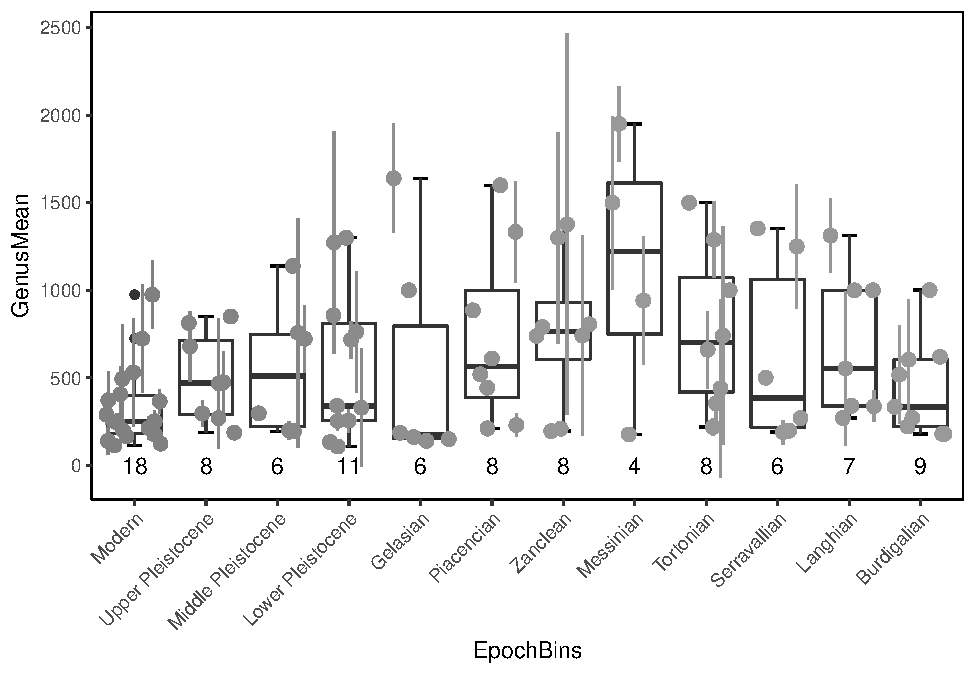
\includegraphics{MA_JJ_files/figure-latex/Boxplots of each genus per time bin-1.pdf}
\caption{Boxplots of mean CL per time bin, including mean and sd CL for
each genus (as pointrange).}
\end{figure}

\newpage

\subsection{continental vs.~insular per time
bin}\label{continental-vs.insular-per-time-bin}

\begin{figure}[htbp]
\centering
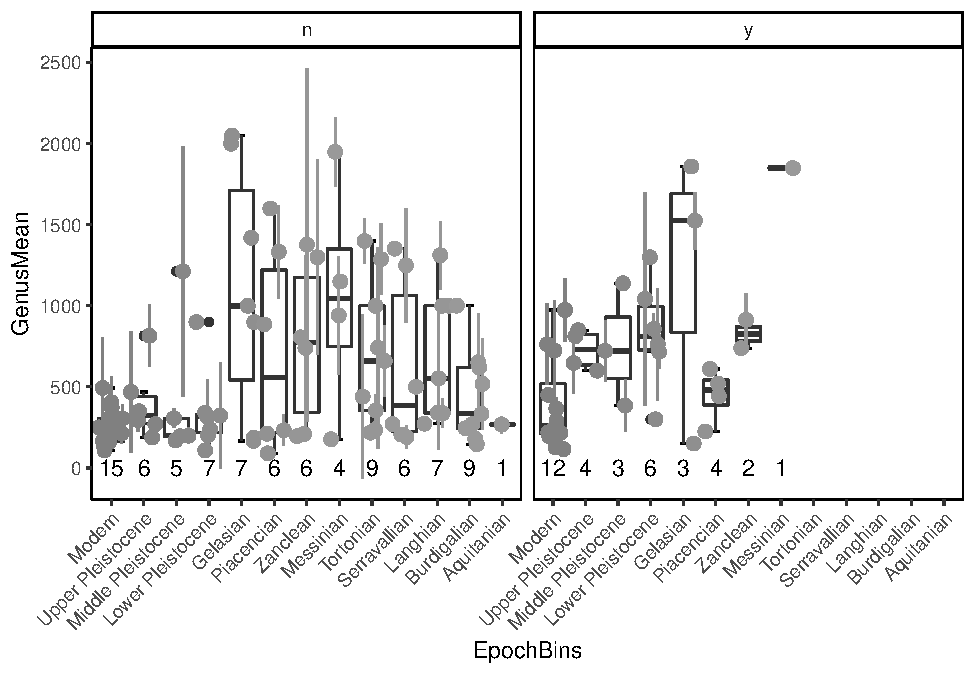
\includegraphics{MA_JJ_files/figure-latex/Boxplots of each genus per time bin, continental vs. insular-1.pdf}
\caption{Boxplots of each genus per time bin, continental vs.~insular
species.}
\end{figure}

\newpage

\subsection{fossil vs.~modern}\label{fossil-vs.modern}

\begin{figure}[htbp]
\centering
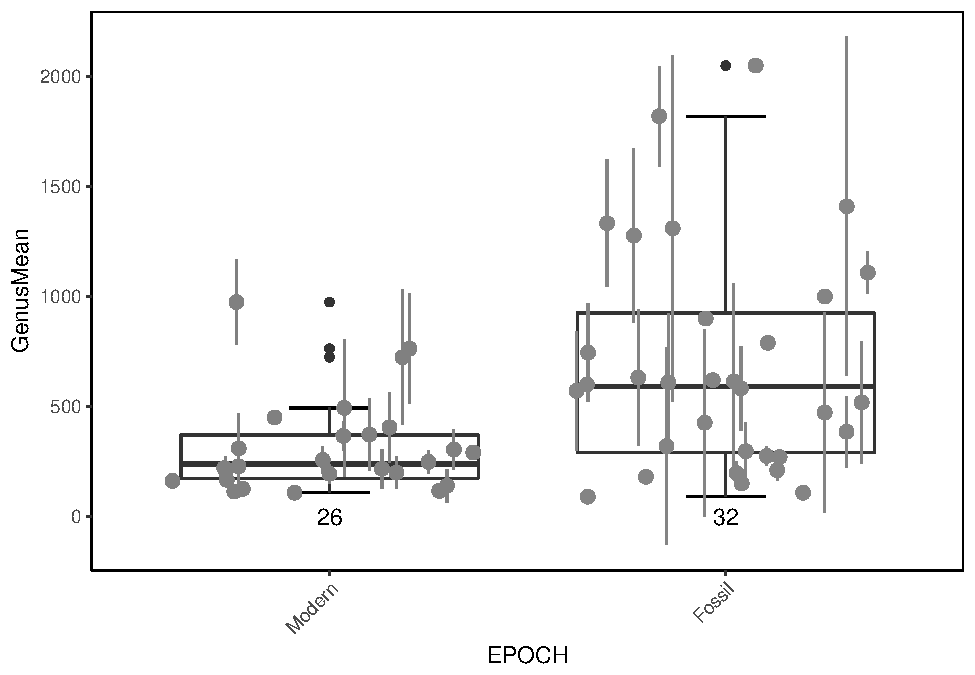
\includegraphics{MA_JJ_files/figure-latex/Boxplots modern vs. fossil-1.pdf}
\caption{Boxplots fossil vs.~modern.}
\end{figure}

\newpage

\subsection{fossil vs.~modern, continental
vs.~insular}\label{fossil-vs.modern-continental-vs.insular}

\begin{figure}[htbp]
\centering
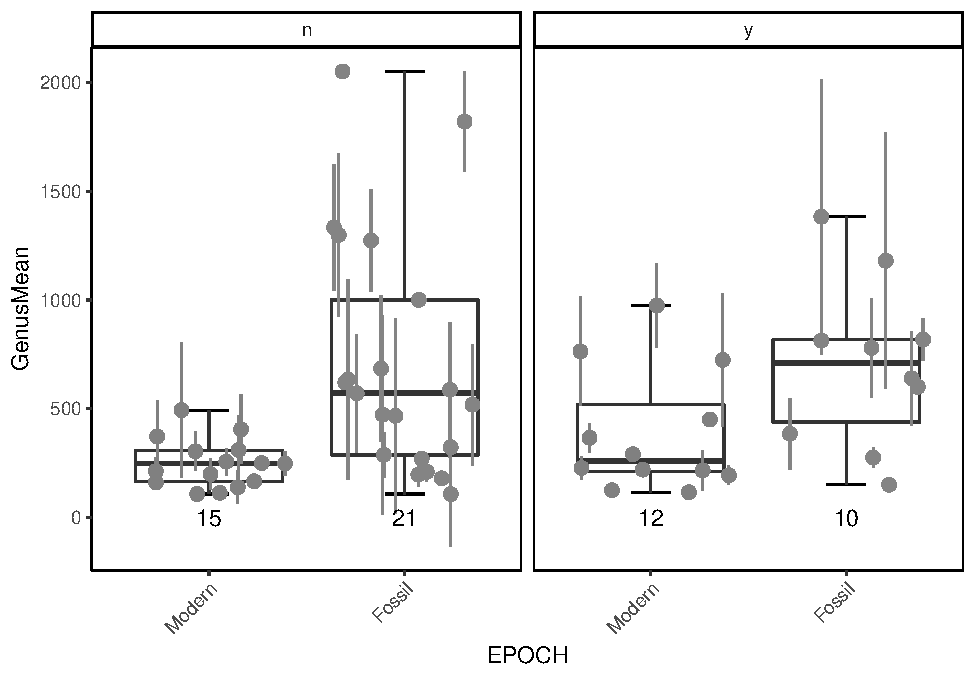
\includegraphics{MA_JJ_files/figure-latex/Boxplots fossil vs. modern, continental vs. insular-1.pdf}
\caption{Boxplots fossil vs.~modern, continental vs.~insular species.}
\end{figure}

\newpage

\subsection{continental vs.~insular}\label{continental-vs.insular-1}

\begin{figure}[htbp]
\centering
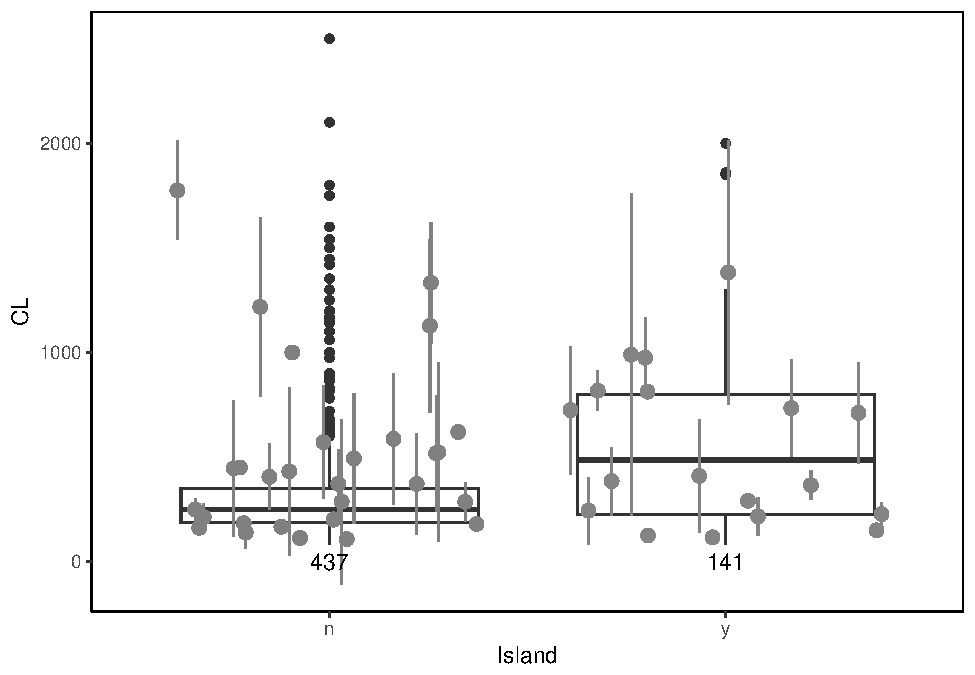
\includegraphics{MA_JJ_files/figure-latex/Boxplot continental vs. insular-1.pdf}
\caption{Boxplot continental vs.~insular, genera summarised}
\end{figure}

\newpage

\subsection{continental vs.~insular per time
bin}\label{continental-vs.insular-per-time-bin-1}

\begin{figure}[htbp]
\centering
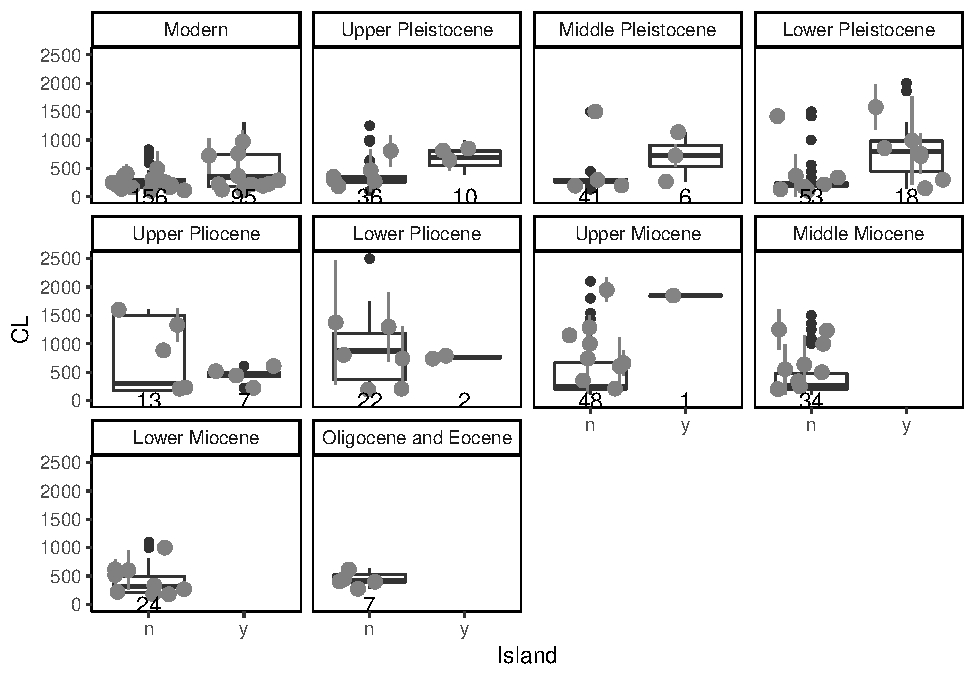
\includegraphics{MA_JJ_files/figure-latex/Boxplot continental vs. insular, split into time bins-1.pdf}
\caption{Boxplot continental vs.~insular, genera summarised}
\end{figure}

\newpage

\subsection{continents}\label{continents-1}

\begin{figure}[htbp]
\centering
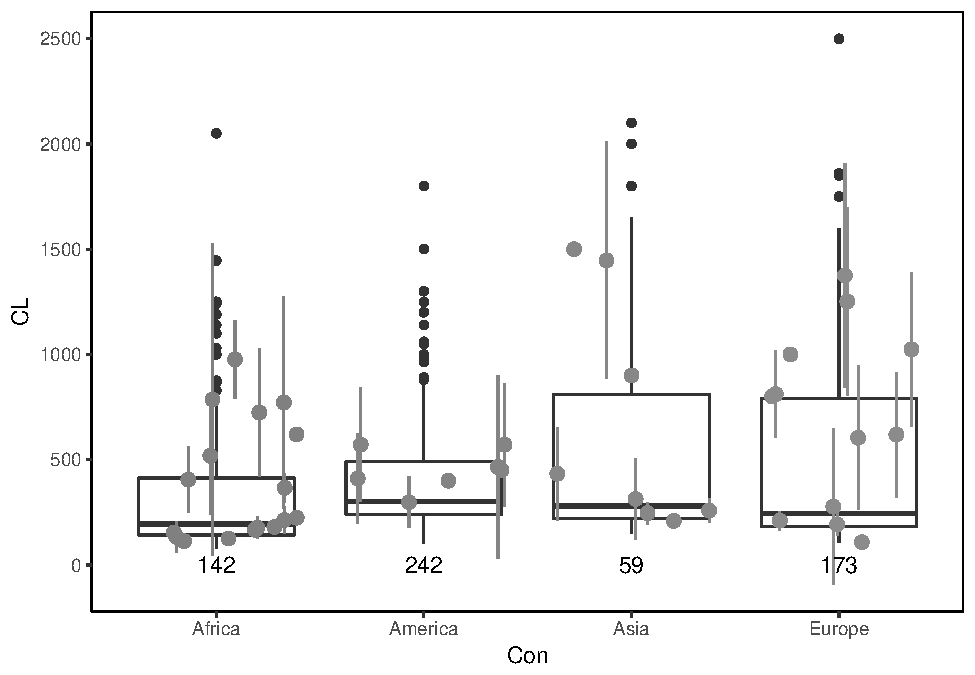
\includegraphics{MA_JJ_files/figure-latex/Boxplot body size split into continents-1.pdf}
\caption{Boxplot: body size on different continents, genera summarised}
\end{figure}

\begin{figure}[htbp]
\centering
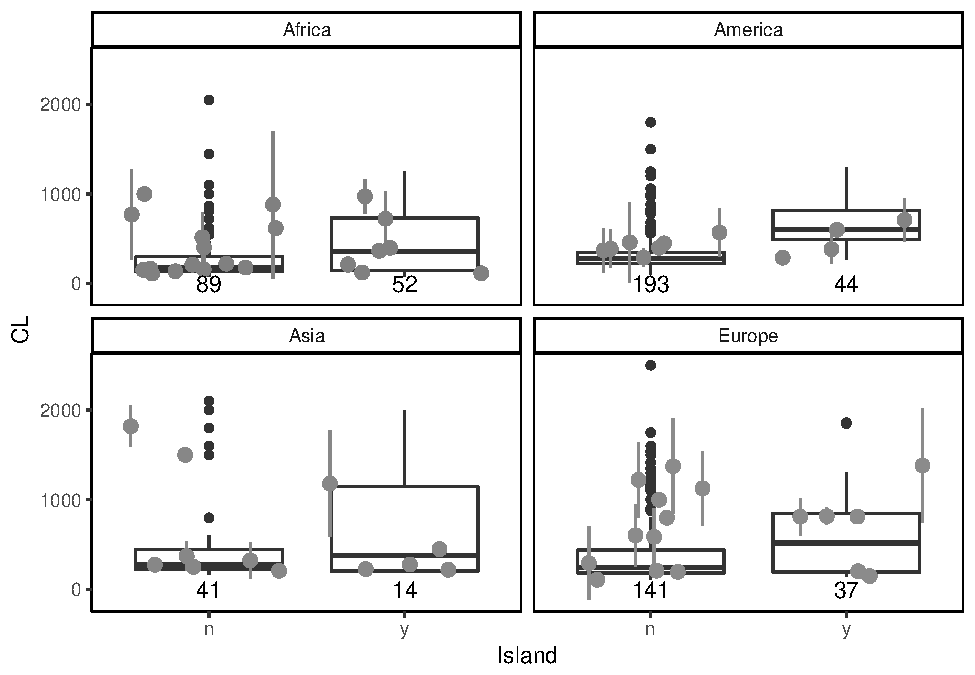
\includegraphics{MA_JJ_files/figure-latex/Boxplot body size split into continents, continental vs. insular-1.pdf}
\caption{Boxplot: body size on different continents, genera summarised}
\end{figure}

\newpage

\section{paleoTS analysis}\label{paleots-analysis}

\subsection{all (continental and
insular)}\label{all-continental-and-insular}

\subsubsection{individuals (all)}\label{individuals-all}

\begin{figure}[htbp]
\centering
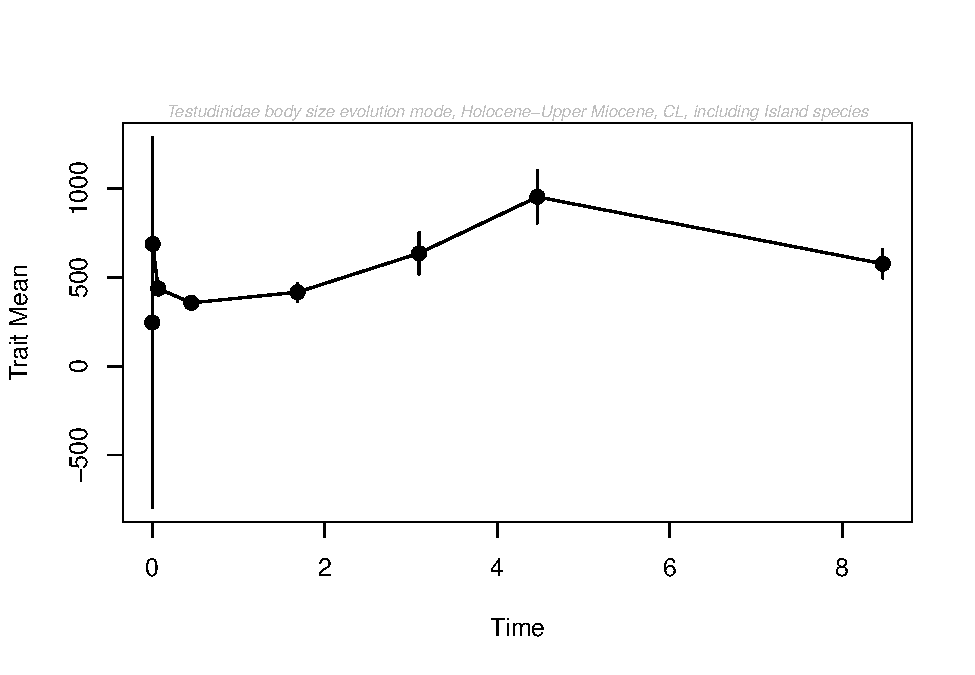
\includegraphics{MA_JJ_files/figure-latex/paleoTS plot-1.pdf}
\caption{individuals, including island species}
\end{figure}

\begin{longtable}[]{@{}lrrrr@{}}
\caption{Model-fitting results for testudinidae, individuals, including
island species}\tabularnewline
\toprule
& logL & K & AICc & Akaike.wt\tabularnewline
\midrule
\endfirsthead
\toprule
& logL & K & AICc & Akaike.wt\tabularnewline
\midrule
\endhead
GRW & -108.0611 & 2 & 221.1221 & 0\tabularnewline
URW & -110.0929 & 1 & 222.4935 & 0\tabularnewline
Stasis & -99.3981 & 2 & 203.7962 & 1\tabularnewline
\bottomrule
\end{longtable}

\begin{longtable}[]{@{}lrrrr@{}}
\caption{Model-fitting results for testudinidae (4 models), individuals,
including island species}\tabularnewline
\toprule
& logL & K & AICc & Akaike.wt\tabularnewline
\midrule
\endfirsthead
\toprule
& logL & K & AICc & Akaike.wt\tabularnewline
\midrule
\endhead
GRW & -108.0611 & 2 & 221.1221 & 0.000\tabularnewline
URW & -110.0929 & 1 & 222.4935 & 0.000\tabularnewline
Stasis & -99.3981 & 2 & 203.7962 & 0.985\tabularnewline
StrictStasis & -104.9433 & 1 & 212.1943 & 0.015\tabularnewline
\bottomrule
\end{longtable}

\newpage

\subsubsection{species (all)}\label{species-all}

\begin{figure}[htbp]
\centering
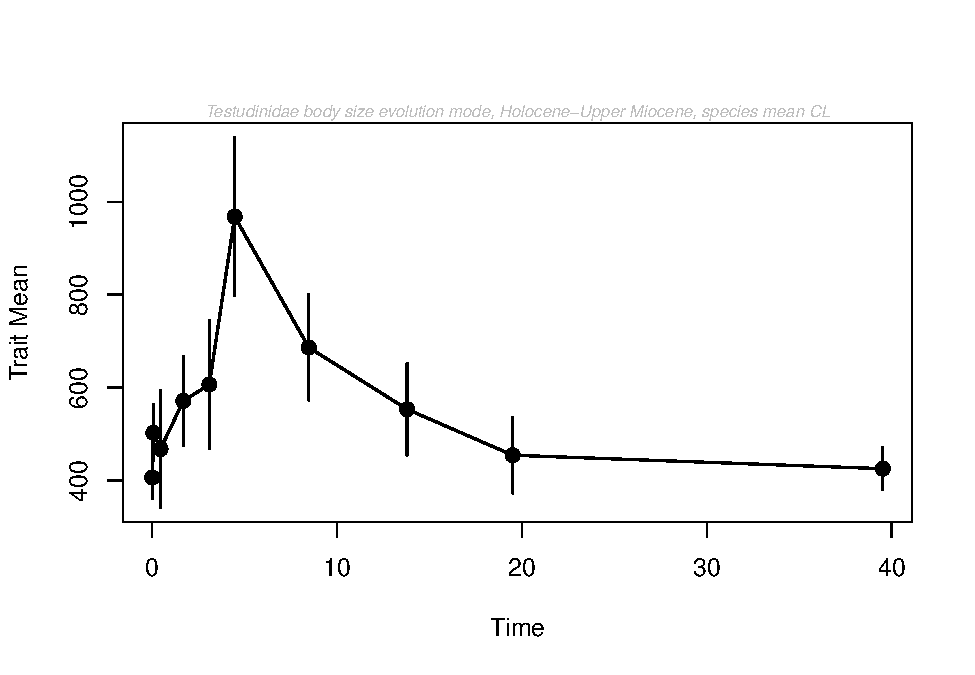
\includegraphics{MA_JJ_files/figure-latex/paleoTS plot with species mean, including island species-1.pdf}
\caption{paleoTS plot with species mean, including island species}
\end{figure}

\begin{longtable}[]{@{}lrrrr@{}}
\caption{Model-fitting results for testudinidae, species, including
island species}\tabularnewline
\toprule
& logL & K & AICc & Akaike.wt\tabularnewline
\midrule
\endfirsthead
\toprule
& logL & K & AICc & Akaike.wt\tabularnewline
\midrule
\endhead
GRW & -94.21080 & 2 & 193.5125 & 0.012\tabularnewline
URW & -94.88189 & 1 & 192.0971 & 0.025\tabularnewline
Stasis & -89.83548 & 2 & 184.7619 & 0.963\tabularnewline
\bottomrule
\end{longtable}

\begin{longtable}[]{@{}lrrrr@{}}
\caption{Model-fitting results for testudinidae (4 models), species,
including island species}\tabularnewline
\toprule
& logL & K & AICc & Akaike.wt\tabularnewline
\midrule
\endfirsthead
\toprule
& logL & K & AICc & Akaike.wt\tabularnewline
\midrule
\endhead
GRW & -94.21080 & 2 & 193.5125 & 0.003\tabularnewline
URW & -94.88189 & 1 & 192.0971 & 0.005\tabularnewline
Stasis & -89.83548 & 2 & 184.7619 & 0.200\tabularnewline
StrictStasis & -89.83548 & 1 & 182.0043 & 0.793\tabularnewline
\bottomrule
\end{longtable}

\newpage

\subsubsection{genera (all)}\label{genera-all}

\begin{figure}[htbp]
\centering
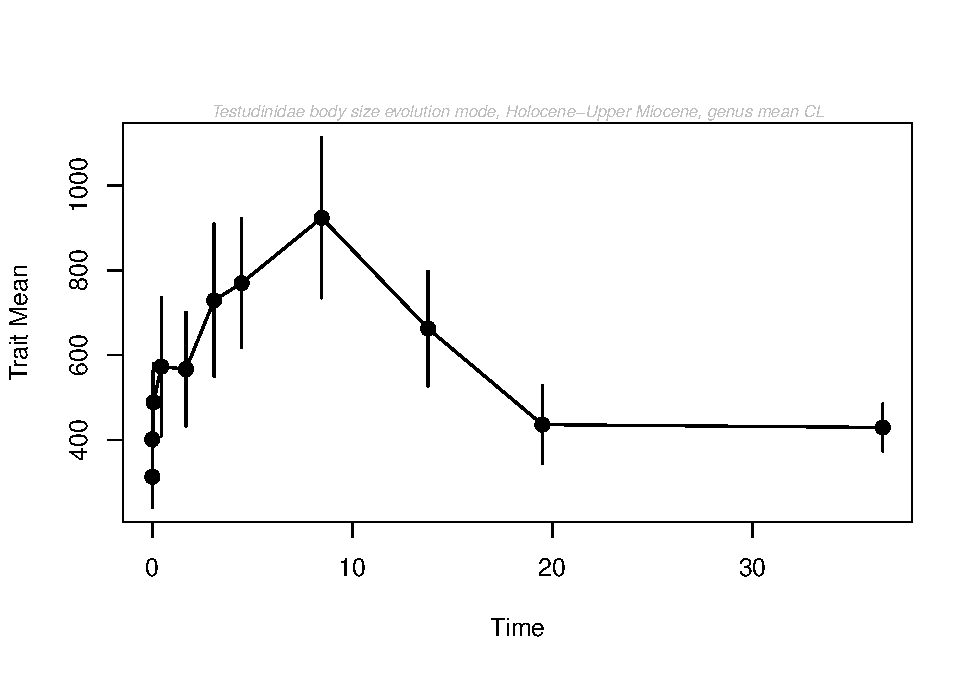
\includegraphics{MA_JJ_files/figure-latex/paleoTS plot with genus mean, including island species-1.pdf}
\caption{paleoTS plot with genus mean, including island species}
\end{figure}

\begin{longtable}[]{@{}lrrrr@{}}
\caption{Model-fitting results for testudinidae, genera, including
island species}\tabularnewline
\toprule
& logL & K & AICc & Akaike.wt\tabularnewline
\midrule
\endfirsthead
\toprule
& logL & K & AICc & Akaike.wt\tabularnewline
\midrule
\endhead
GRW & -101.51384 & 2 & 208.0277 & 0.087\tabularnewline
URW & -101.95549 & 1 & 206.2187 & 0.215\tabularnewline
Stasis & -99.43342 & 2 & 203.8668 & 0.698\tabularnewline
\bottomrule
\end{longtable}

\begin{longtable}[]{@{}lrrrr@{}}
\caption{Model-fitting results for testudinidae (4 models), genera,
including island species}\tabularnewline
\toprule
& logL & K & AICc & Akaike.wt\tabularnewline
\midrule
\endfirsthead
\toprule
& logL & K & AICc & Akaike.wt\tabularnewline
\midrule
\endhead
GRW & -101.51384 & 2 & 208.0277 & 0.083\tabularnewline
URW & -101.95549 & 1 & 206.2187 & 0.204\tabularnewline
Stasis & -99.43342 & 2 & 203.8668 & 0.662\tabularnewline
StrictStasis & -103.34048 & 1 & 208.9887 & 0.051\tabularnewline
\bottomrule
\end{longtable}

\newpage

\subsection{continental (excluding insular
species)}\label{continental-excluding-insular-species}

\subsubsection{individuals (continental)}\label{individuals-continental}

\begin{figure}[htbp]
\centering
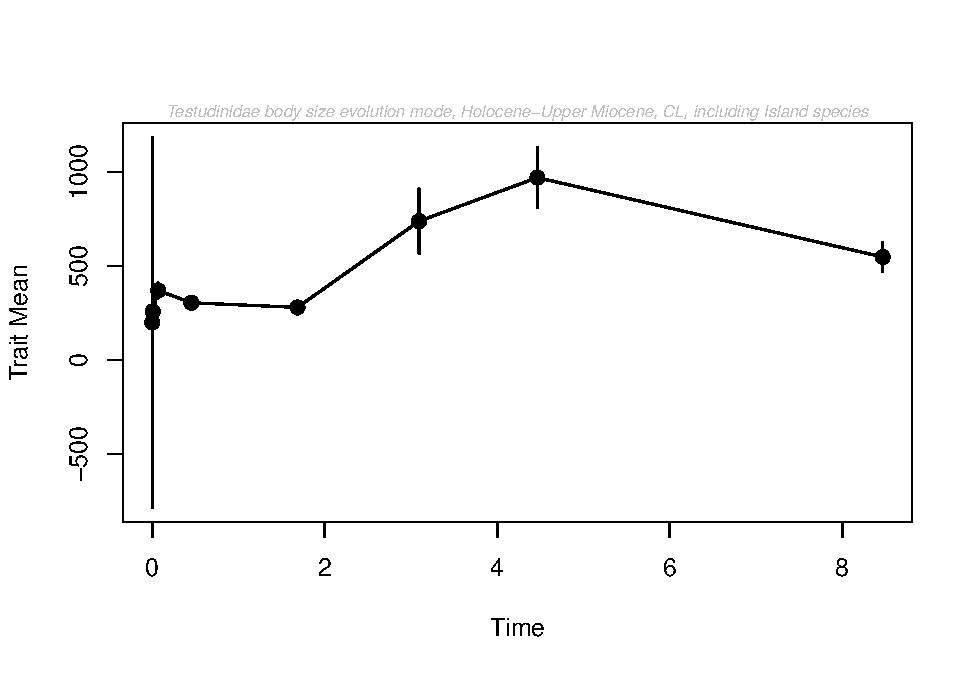
\includegraphics{MA_JJ_files/figure-latex/paleoTS, individuals, exluding island species-1.pdf}
\caption{individuals, excluding island species}
\end{figure}

\begin{longtable}[]{@{}lrrrr@{}}
\caption{Model-fitting results for testudinidae, individuals, excluding
island species}\tabularnewline
\toprule
& logL & K & AICc & Akaike.wt\tabularnewline
\midrule
\endfirsthead
\toprule
& logL & K & AICc & Akaike.wt\tabularnewline
\midrule
\endhead
GRW & -108.8712 & 2 & 222.7424 & 0.001\tabularnewline
URW & -109.1051 & 1 & 220.5179 & 0.004\tabularnewline
Stasis & -102.2252 & 2 & 209.4504 & 0.995\tabularnewline
\bottomrule
\end{longtable}

\begin{longtable}[]{@{}lrrrr@{}}
\caption{Model-fitting results for testudinidae (4 models), individuals,
excluding island species}\tabularnewline
\toprule
& logL & K & AICc & Akaike.wt\tabularnewline
\midrule
\endfirsthead
\toprule
& logL & K & AICc & Akaike.wt\tabularnewline
\midrule
\endhead
GRW & -108.8712 & 2 & 222.7424 & 0.001\tabularnewline
URW & -109.1051 & 1 & 220.5179 & 0.004\tabularnewline
Stasis & -102.2252 & 2 & 209.4504 & 0.995\tabularnewline
StrictStasis & -117.2903 & 1 & 236.8882 & 0.000\tabularnewline
\bottomrule
\end{longtable}

\newpage

\subsubsection{species (continental)}\label{species-continental}

\begin{figure}[htbp]
\centering
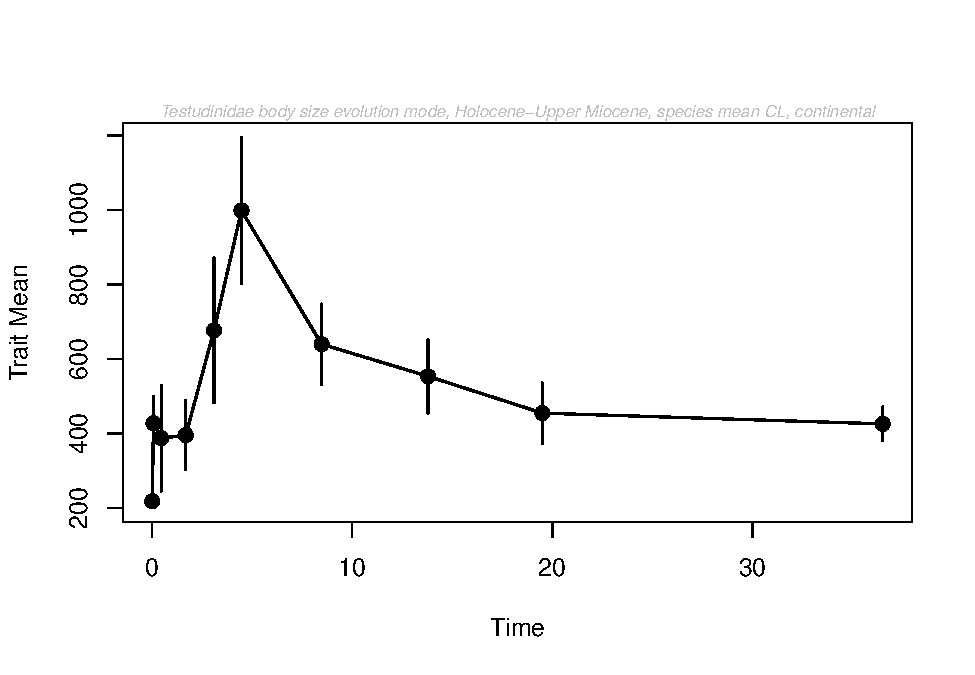
\includegraphics{MA_JJ_files/figure-latex/paleoTS plot with species mean, excluding island species-1.pdf}
\caption{paleoTS plot with species mean, excluding island species}
\end{figure}

\begin{longtable}[]{@{}lrrrr@{}}
\caption{Model-fitting results for testudinidae, species, excluding
island species}\tabularnewline
\toprule
& logL & K & AICc & Akaike.wt\tabularnewline
\midrule
\endfirsthead
\toprule
& logL & K & AICc & Akaike.wt\tabularnewline
\midrule
\endhead
GRW & -97.35309 & 2 & 199.7971 & 0.004\tabularnewline
URW & -97.72768 & 1 & 197.7887 & 0.010\tabularnewline
Stasis & -91.78052 & 2 & 188.6519 & 0.986\tabularnewline
\bottomrule
\end{longtable}

\begin{longtable}[]{@{}lrrrr@{}}
\caption{Model-fitting results for testudinidae, species, excluding
island species}\tabularnewline
\toprule
& logL & K & AICc & Akaike.wt\tabularnewline
\midrule
\endfirsthead
\toprule
& logL & K & AICc & Akaike.wt\tabularnewline
\midrule
\endhead
GRW & -97.35309 & 2 & 199.7971 & 0.001\tabularnewline
URW & -97.72768 & 1 & 197.7887 & 0.002\tabularnewline
Stasis & -91.78052 & 2 & 188.6519 & 0.201\tabularnewline
StrictStasis & -91.78052 & 1 & 185.8944 & 0.797\tabularnewline
\bottomrule
\end{longtable}

\newpage

\subsubsection{genera (continental)}\label{genera-continental}

\begin{figure}[htbp]
\centering
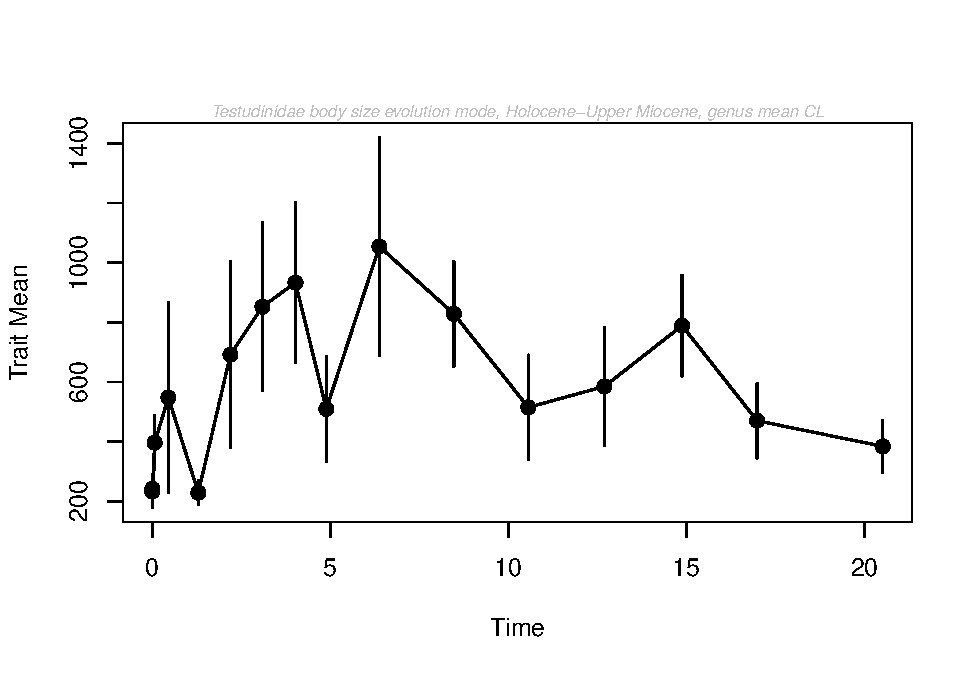
\includegraphics{MA_JJ_files/figure-latex/paleoTS plot with genus mean, excluding island species-1.pdf}
\caption{paleoTS plot with genus mean, excluding island species}
\end{figure}

\begin{longtable}[]{@{}lrrrr@{}}
\caption{Model-fitting results for testudinidae, genera, excluding
insular species}\tabularnewline
\toprule
& logL & K & AICc & Akaike.wt\tabularnewline
\midrule
\endfirsthead
\toprule
& logL & K & AICc & Akaike.wt\tabularnewline
\midrule
\endhead
GRW & -103.2958 & 2 & 211.5916 & 0.251\tabularnewline
URW & -103.9853 & 1 & 210.2784 & 0.484\tabularnewline
Stasis & -103.2385 & 2 & 211.4769 & 0.266\tabularnewline
\bottomrule
\end{longtable}

\begin{longtable}[]{@{}lrrrr@{}}
\caption{Model-fitting results for testudinidae, genera, excluding
insular species}\tabularnewline
\toprule
& logL & K & AICc & Akaike.wt\tabularnewline
\midrule
\endfirsthead
\toprule
& logL & K & AICc & Akaike.wt\tabularnewline
\midrule
\endhead
GRW & -103.2958 & 2 & 211.5916 & 0.251\tabularnewline
URW & -103.9853 & 1 & 210.2784 & 0.484\tabularnewline
Stasis & -103.2385 & 2 & 211.4769 & 0.266\tabularnewline
StrictStasis & -112.5911 & 1 & 227.4899 & 0.000\tabularnewline
\bottomrule
\end{longtable}

\newpage

\subsection{insular (excluding
continental)}\label{insular-excluding-continental}

\subsubsection{individuals (insular)}\label{individuals-insular}

\begin{figure}[htbp]
\centering
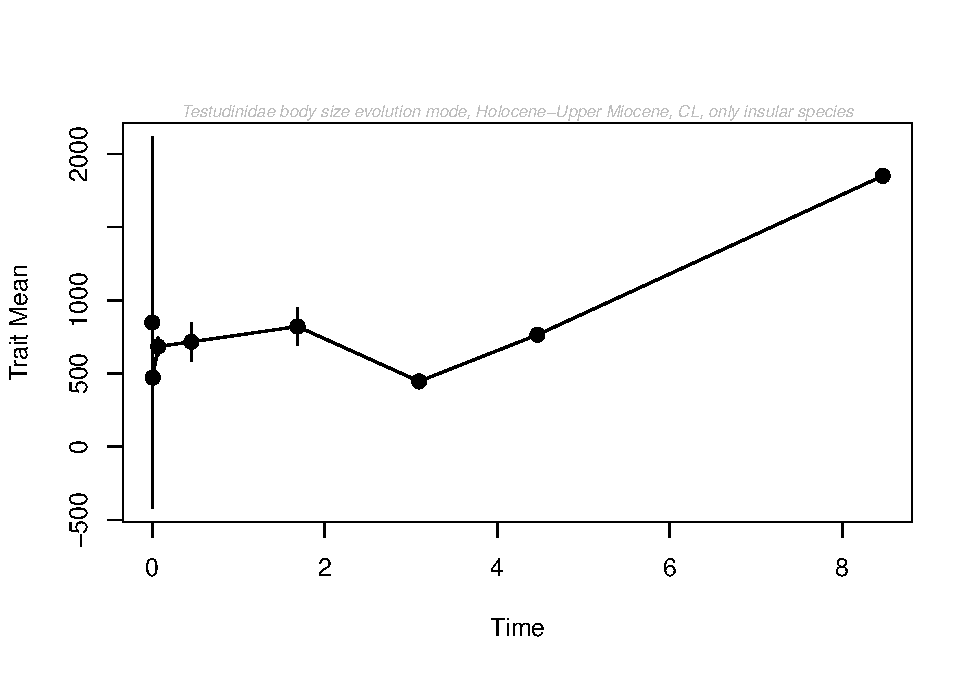
\includegraphics{MA_JJ_files/figure-latex/paleoTS, individuals, exluding continental species-1.pdf}
\caption{individuals, excluding continental species}
\end{figure}

\begin{longtable}[]{@{}lrrrr@{}}
\caption{Model-fitting results for testudinidae, individuals, only
insular species}\tabularnewline
\toprule
& logL & K & AICc & Akaike.wt\tabularnewline
\midrule
\endfirsthead
\toprule
& logL & K & AICc & Akaike.wt\tabularnewline
\midrule
\endhead
GRW & -70.13930 & 2 & 146.2786 & 0.044\tabularnewline
URW & -71.84375 & 1 & 146.2589 & 0.044\tabularnewline
Stasis & -67.09727 & 2 & 140.1945 & 0.912\tabularnewline
\bottomrule
\end{longtable}

\newpage

\subsubsection{species (insular)}\label{species-insular}

\begin{figure}[htbp]
\centering
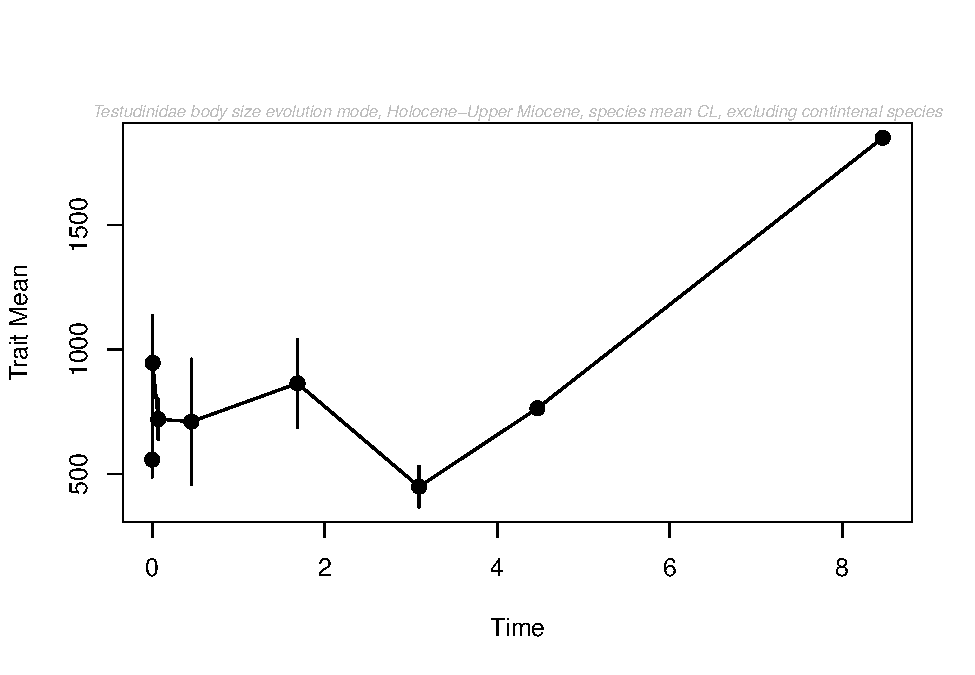
\includegraphics{MA_JJ_files/figure-latex/paleoTS plot with species mean, excluding continental species-1.pdf}
\caption{paleoTS plot with species mean, only insular species}
\end{figure}

\begin{longtable}[]{@{}lrrrr@{}}
\caption{Model-fitting results for testudinidae, species, only insular
species}\tabularnewline
\toprule
& logL & K & AICc & Akaike.wt\tabularnewline
\midrule
\endfirsthead
\toprule
& logL & K & AICc & Akaike.wt\tabularnewline
\midrule
\endhead
GRW & -57.04948 & 2 & 120.4990 & 0.84\tabularnewline
URW & -60.94771 & 1 & 124.5621 & 0.11\tabularnewline
Stasis & -59.87110 & 2 & 126.1422 & 0.05\tabularnewline
\bottomrule
\end{longtable}

\newpage

\subsubsection{genera (insular)}\label{genera-insular}

\begin{figure}[htbp]
\centering
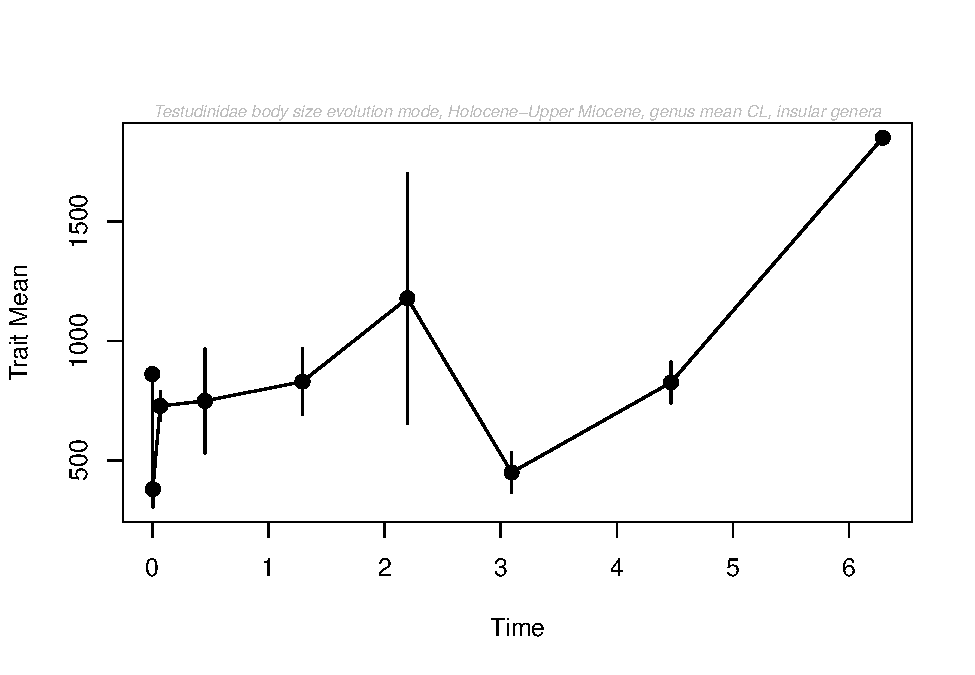
\includegraphics{MA_JJ_files/figure-latex/paleoTS plot with genus mean, excluding continental species-1.pdf}
\caption{paleoTS plot with genus mean, only insular species}
\end{figure}

\begin{longtable}[]{@{}lrrrr@{}}
\caption{Model-fitting results for testudinidae, genera, only insular
species}\tabularnewline
\toprule
& logL & K & AICc & Akaike.wt\tabularnewline
\midrule
\endfirsthead
\toprule
& logL & K & AICc & Akaike.wt\tabularnewline
\midrule
\endhead
GRW & -76.60847 & 2 & 159.2169 & 0\tabularnewline
URW & -84.13413 & 1 & 170.8397 & 0\tabularnewline
Stasis & -67.41721 & 2 & 140.8344 & 1\tabularnewline
\bottomrule
\end{longtable}

\newpage

\subsection{play with time bins: no bins (mean age of each sample ==
tt)}\label{play-with-time-bins-no-bins-mean-age-of-each-sample-tt}

\subsubsection{all}\label{all-1}

\begin{figure}[htbp]
\centering
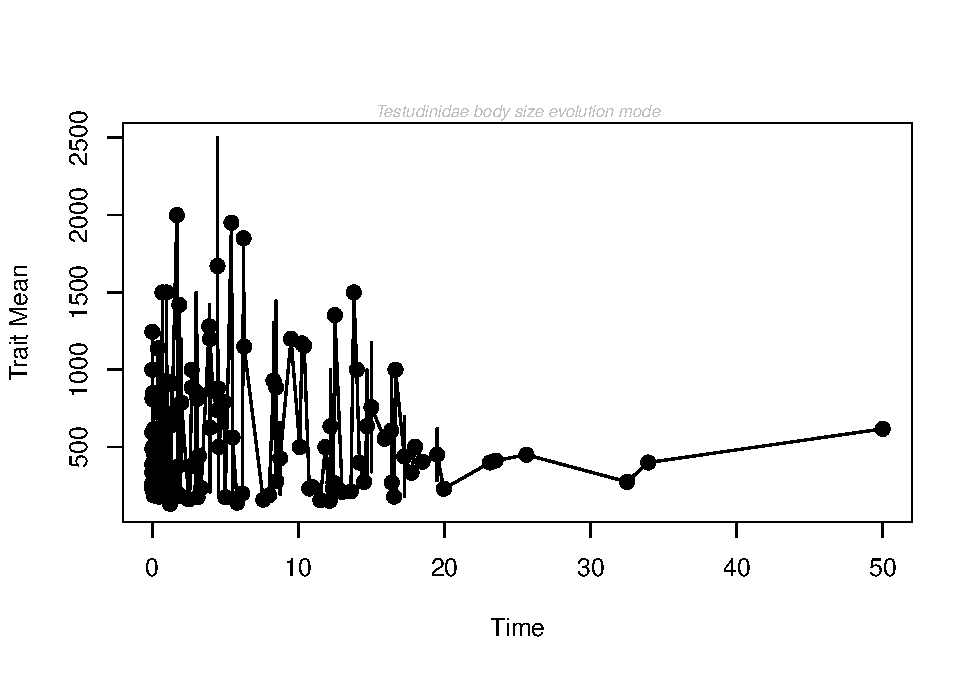
\includegraphics{MA_JJ_files/figure-latex/paleoTS with different time bins, no bins, genera-1.pdf}
\caption{Mean age of each sample as time bin, genera}
\end{figure}

\begin{longtable}[]{@{}lrrrr@{}}
\caption{Model-fitting results for testudinidae, no bins,
genera}\tabularnewline
\toprule
& logL & K & AICc & Akaike.wt\tabularnewline
\midrule
\endfirsthead
\toprule
& logL & K & AICc & Akaike.wt\tabularnewline
\midrule
\endhead
GRW & -6948.0075 & 2 & 13900.126 & 0\tabularnewline
URW & -8243.1398 & 1 & 16488.316 & 0\tabularnewline
Stasis & -885.7773 & 2 & 1775.666 & 1\tabularnewline
\bottomrule
\end{longtable}

\newpage

\subsubsection{continental (no bins)}\label{continental-no-bins}

\begin{figure}[htbp]
\centering
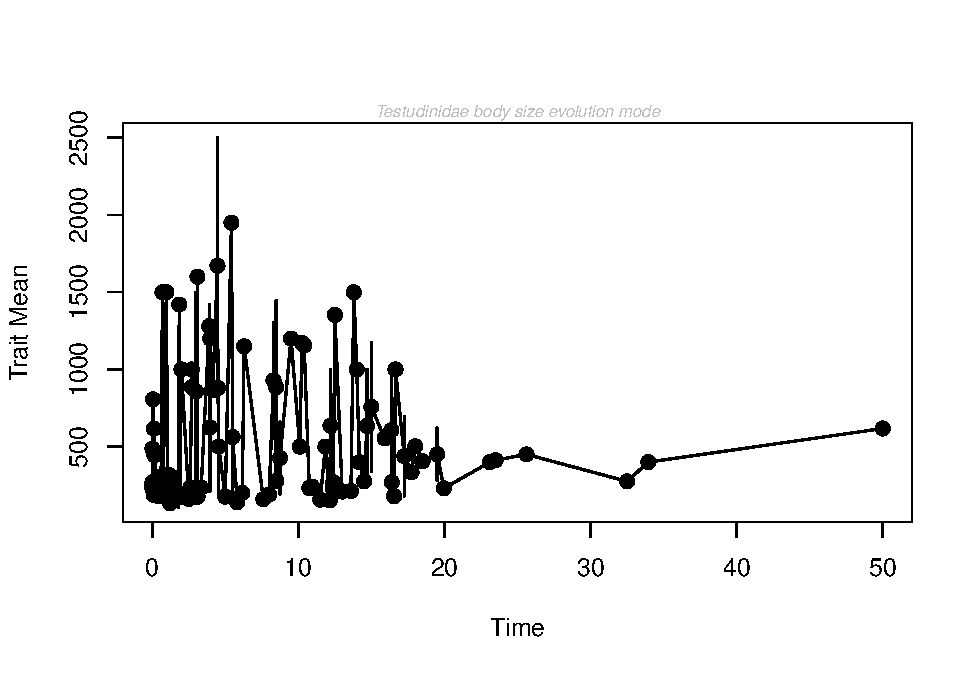
\includegraphics{MA_JJ_files/figure-latex/paleoTS with different time bins, no bins, genera, continental-1.pdf}
\caption{Mean age of each sample as time bin, genera, continental}
\end{figure}

\begin{longtable}[]{@{}lrrrr@{}}
\caption{Model-fitting results for testudinidae, no bins, genera,
continental}\tabularnewline
\toprule
& logL & K & AICc & Akaike.wt\tabularnewline
\midrule
\endfirsthead
\toprule
& logL & K & AICc & Akaike.wt\tabularnewline
\midrule
\endhead
GRW & -782.8522 & 2 & 1569.836 & 0\tabularnewline
URW & -782.8541 & 1 & 1567.752 & 0\tabularnewline
Stasis & -704.9241 & 2 & 1413.980 & 1\tabularnewline
\bottomrule
\end{longtable}

\newpage

\subsubsection{insular (no bins)}\label{insular-no-bins}

\begin{figure}[htbp]
\centering
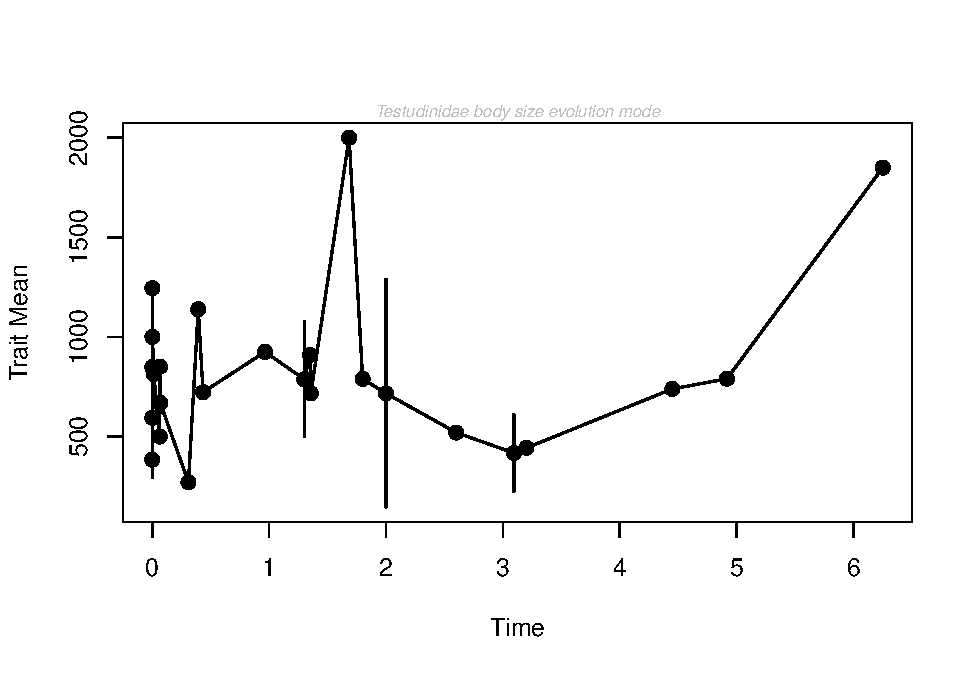
\includegraphics{MA_JJ_files/figure-latex/paleoTS with different time bins, no bins, genera, insular-1.pdf}
\caption{Mean age of each sample as time bin, genera, insular}
\end{figure}

\begin{longtable}[]{@{}lrrrr@{}}
\caption{Model-fitting results for testudinidae, no bins, genera,
insular}\tabularnewline
\toprule
& logL & K & AICc & Akaike.wt\tabularnewline
\midrule
\endfirsthead
\toprule
& logL & K & AICc & Akaike.wt\tabularnewline
\midrule
\endhead
GRW & -3723.151 & 2 & 7450.8734 & 0\tabularnewline
URW & -11230.978 & 1 & 22464.1373 & 0\tabularnewline
Stasis & -187.450 & 2 & 379.4714 & 1\tabularnewline
\bottomrule
\end{longtable}

\newpage

\subsection{Equal time bins}\label{equal-time-bins}

\subsubsection{individuals (equal bins)}\label{individuals-equal-bins}

\begin{figure}[htbp]
\centering
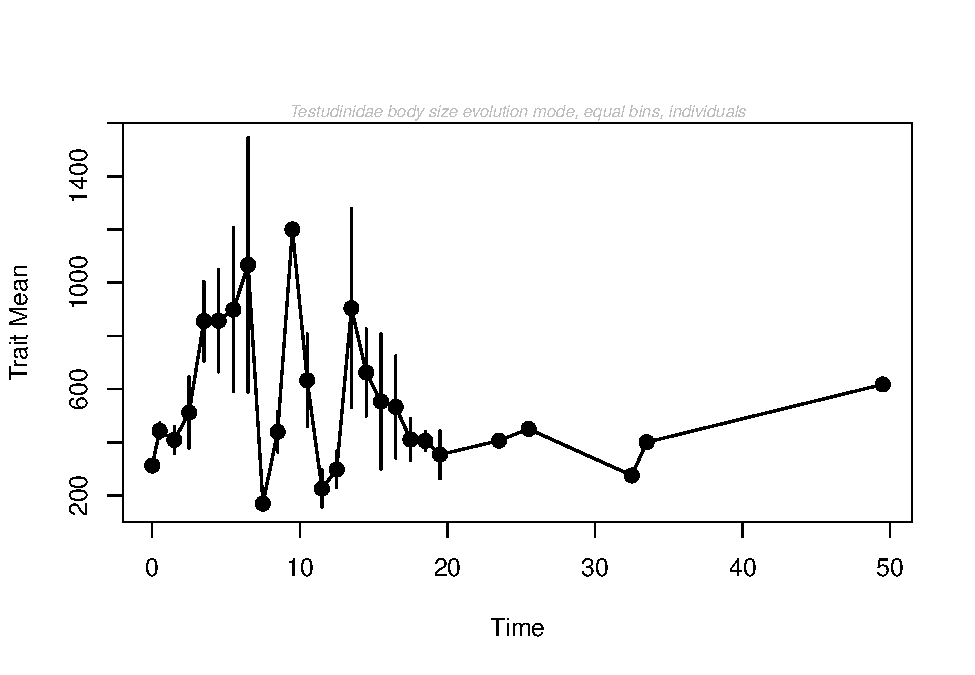
\includegraphics{MA_JJ_files/figure-latex/Play around with time bins, larger equal bins, individuals-1.pdf}
\caption{Equal bins, individuals}
\end{figure}

\begin{longtable}[]{@{}lrrrr@{}}
\caption{Model-fitting results for testudinidae, equal time bins,
individuals}\tabularnewline
\toprule
& logL & K & AICc & Akaike.wt\tabularnewline
\midrule
\endfirsthead
\toprule
& logL & K & AICc & Akaike.wt\tabularnewline
\midrule
\endhead
GRW & -181.0860 & 2 & 366.7174 & 0.001\tabularnewline
URW & -182.5837 & 1 & 367.3413 & 0.001\tabularnewline
Stasis & -174.2101 & 2 & 352.9656 & 0.998\tabularnewline
\bottomrule
\end{longtable}

\newpage

\subsubsection{species (equal bins)}\label{species-equal-bins}

\begin{figure}[htbp]
\centering
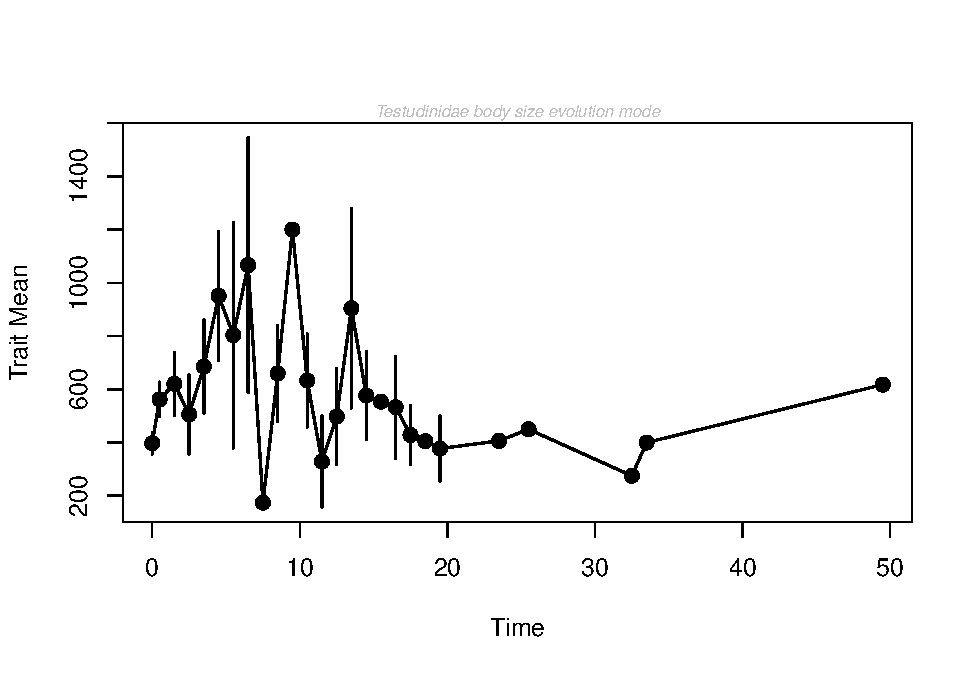
\includegraphics{MA_JJ_files/figure-latex/Play around with time bins, equal bin, species level-1.pdf}
\caption{Equal bins, species}
\end{figure}

\begin{longtable}[]{@{}lrrrr@{}}
\caption{Model-fitting results for testudinidae, equal time bins,
species}\tabularnewline
\toprule
& logL & K & AICc & Akaike.wt\tabularnewline
\midrule
\endfirsthead
\toprule
& logL & K & AICc & Akaike.wt\tabularnewline
\midrule
\endhead
GRW & -177.3909 & 2 & 359.3272 & 0.011\tabularnewline
URW & -178.7626 & 1 & 359.6991 & 0.010\tabularnewline
Stasis & -172.9454 & 2 & 350.4363 & 0.979\tabularnewline
\bottomrule
\end{longtable}

\newpage

\subsubsection{genera (equal bins)}\label{genera-equal-bins}

\begin{figure}[htbp]
\centering
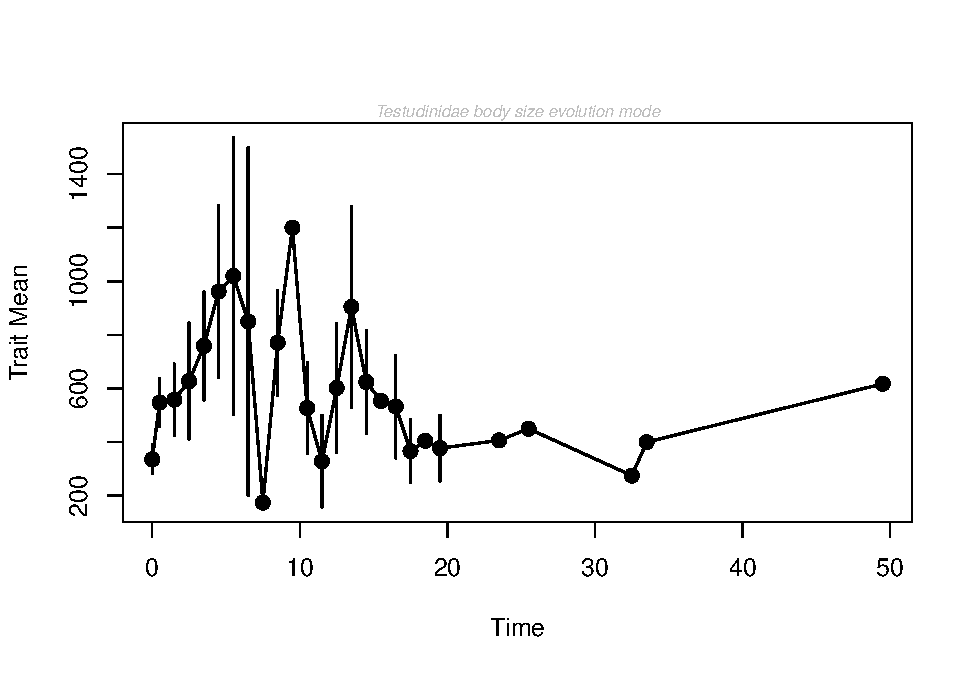
\includegraphics{MA_JJ_files/figure-latex/Play around with time bins, generic level-1.pdf}
\caption{Equal bins, genera}
\end{figure}

\begin{longtable}[]{@{}lrrrr@{}}
\caption{Model-fitting results for testudinidae, equal time bins,
genera}\tabularnewline
\toprule
& logL & K & AICc & Akaike.wt\tabularnewline
\midrule
\endfirsthead
\toprule
& logL & K & AICc & Akaike.wt\tabularnewline
\midrule
\endhead
GRW & -179.4504 & 2 & 363.4462 & 0.008\tabularnewline
URW & -178.8180 & 1 & 359.8099 & 0.051\tabularnewline
Stasis & -174.7233 & 2 & 353.9921 & 0.940\tabularnewline
\bottomrule
\end{longtable}

\newpage

\subsection{larger equal bins}\label{larger-equal-bins}

\subsubsection{genera (larger equal
bins)}\label{genera-larger-equal-bins}

\begin{figure}[htbp]
\centering
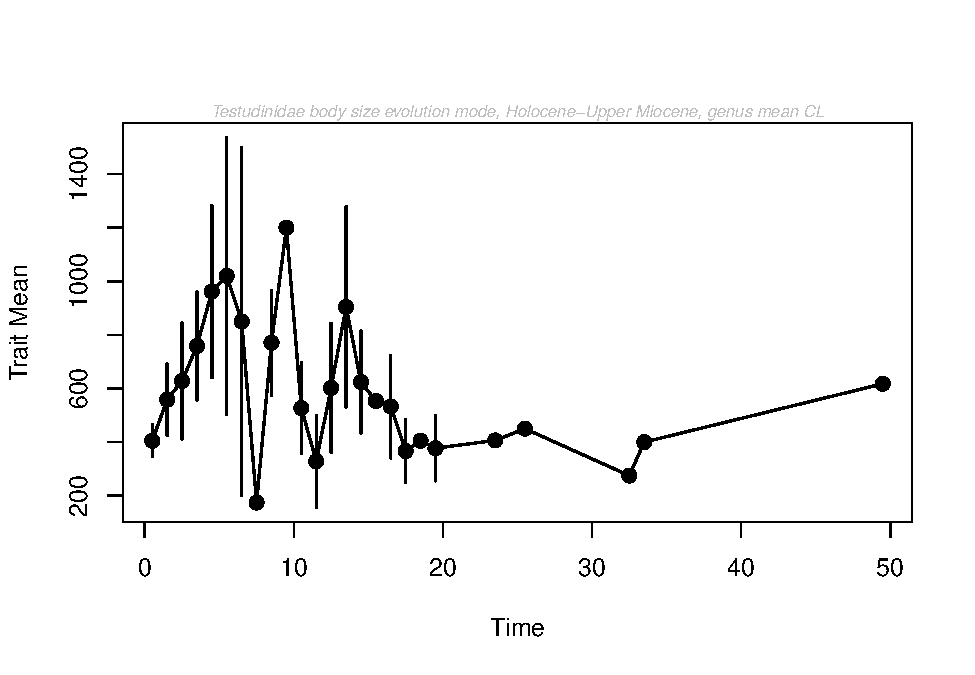
\includegraphics{MA_JJ_files/figure-latex/Play around with larger time bins, generic level-1.pdf}
\caption{Larger equal bins, genera}
\end{figure}

\begin{longtable}[]{@{}lrrrr@{}}
\caption{Model-fitting results for testudinidae, larger equal time bins,
genera}\tabularnewline
\toprule
& logL & K & AICc & Akaike.wt\tabularnewline
\midrule
\endfirsthead
\toprule
& logL & K & AICc & Akaike.wt\tabularnewline
\midrule
\endhead
GRW & -172.6279 & 2 & 349.8272 & 0.036\tabularnewline
URW & -172.9972 & 1 & 348.1763 & 0.082\tabularnewline
Stasis & -169.4260 & 2 & 343.4234 & 0.882\tabularnewline
\bottomrule
\end{longtable}

\newpage

\subsection{per continent}\label{per-continent}

\subsubsection{Africa, individuals}\label{africa-individuals}

\begin{figure}[htbp]
\centering
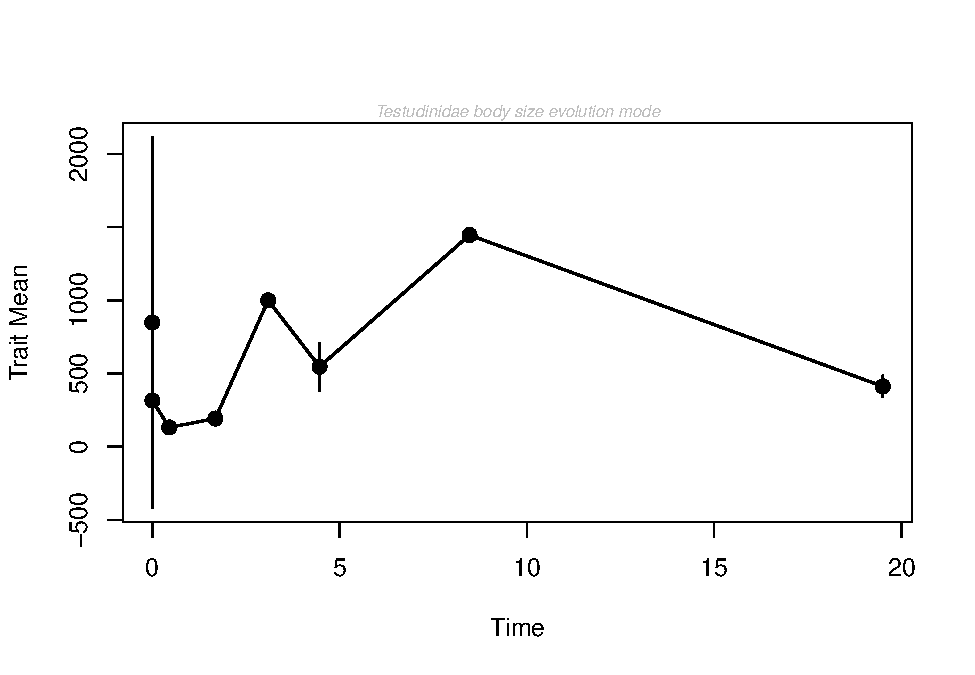
\includegraphics{MA_JJ_files/figure-latex/paleoTS, individuals, Africa-1.pdf}
\caption{Africa, individuals}
\end{figure}

\begin{longtable}[]{@{}lrrrr@{}}
\caption{Model-fitting results for testudinidae, individuals,
Africa}\tabularnewline
\toprule
& logL & K & AICc & Akaike.wt\tabularnewline
\midrule
\endfirsthead
\toprule
& logL & K & AICc & Akaike.wt\tabularnewline
\midrule
\endhead
GRW & -78.43610 & 2 & 162.8722 & 0\tabularnewline
URW & -81.12817 & 1 & 164.8278 & 0\tabularnewline
Stasis & -67.24042 & 2 & 140.4808 & 1\tabularnewline
\bottomrule
\end{longtable}

\newpage 

\subsubsection{Africa, no bins,
individuals}\label{africa-no-bins-individuals}

\begin{figure}[htbp]
\centering
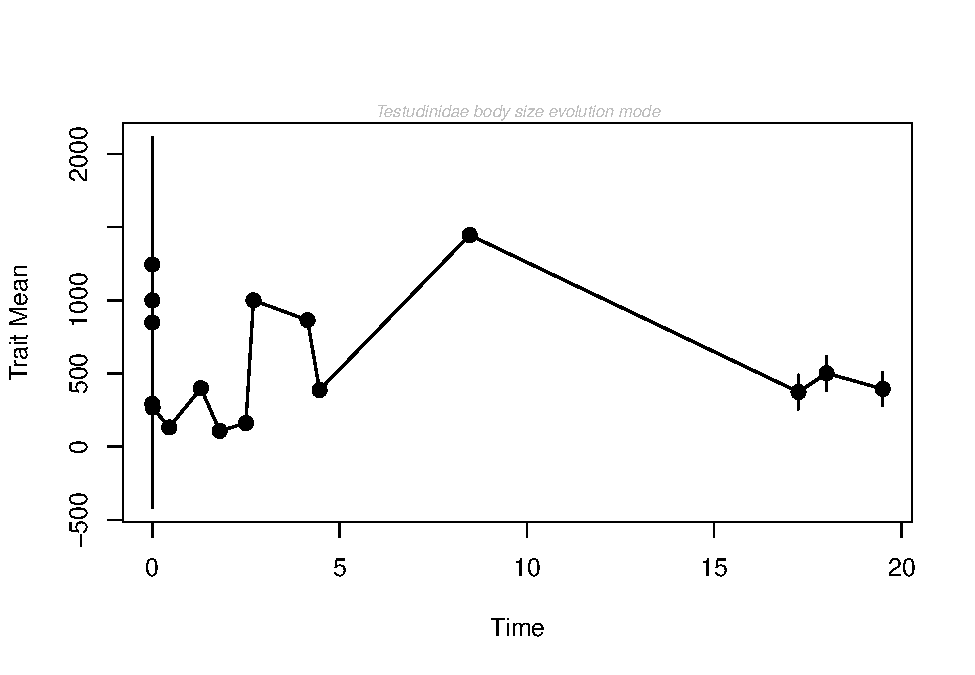
\includegraphics{MA_JJ_files/figure-latex/paleoTS, no bins individuals, Africa-1.pdf}
\caption{Africa, individuals, no bins}
\end{figure}

\begin{longtable}[]{@{}lrrrr@{}}
\caption{Model-fitting results for testudinidae, individuals, no bins,
Africa}\tabularnewline
\toprule
& logL & K & AICc & Akaike.wt\tabularnewline
\midrule
\endfirsthead
\toprule
& logL & K & AICc & Akaike.wt\tabularnewline
\midrule
\endhead
GRW & -1025.9662 & 2 & 2056.9323 & 0\tabularnewline
URW & -2572.3987 & 1 & 5147.1052 & 0\tabularnewline
Stasis & -130.7568 & 2 & 266.5135 & 1\tabularnewline
\bottomrule
\end{longtable}

\newpage 

\subsubsection{Africa, no bins, genera}\label{africa-no-bins-genera}

\begin{figure}[htbp]
\centering
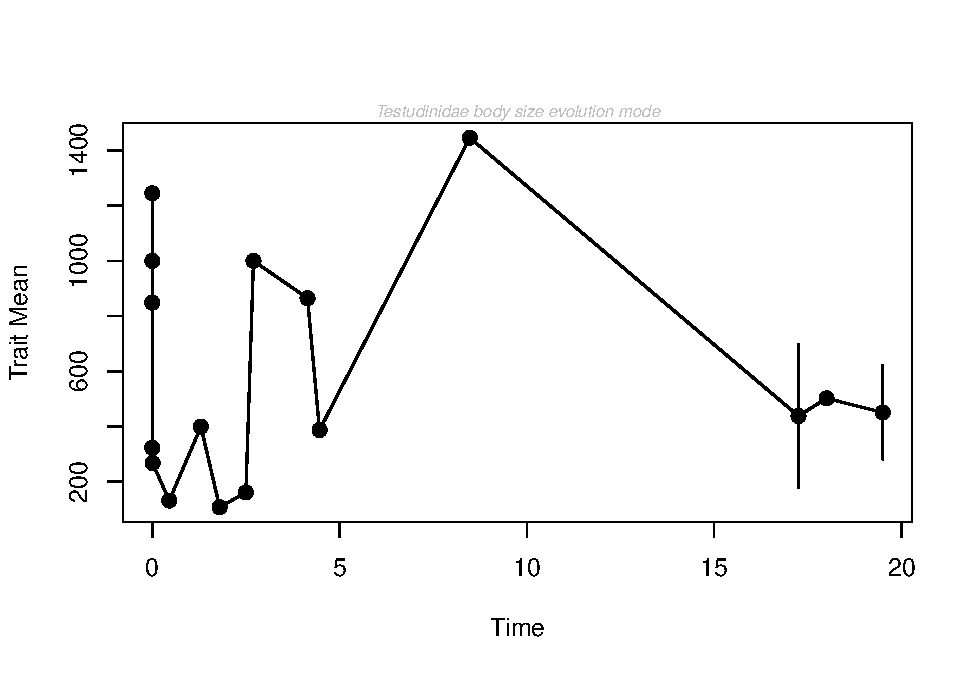
\includegraphics{MA_JJ_files/figure-latex/paleoTS with different time bins, no bins, genera, Africa-1.pdf}
\caption{Mean age of each sample as time bin, genera, Africa}
\end{figure}

\begin{longtable}[]{@{}lrrrr@{}}
\caption{Model-fitting results for testudinidae, no bins,
genera}\tabularnewline
\toprule
& logL & K & AICc & Akaike.wt\tabularnewline
\midrule
\endfirsthead
\toprule
& logL & K & AICc & Akaike.wt\tabularnewline
\midrule
\endhead
GRW & -221.6685 & 2 & 448.3369 & 0\tabularnewline
URW & -167.7116 & 1 & 337.7309 & 0\tabularnewline
Stasis & -111.6921 & 2 & 228.3842 & 1\tabularnewline
\bottomrule
\end{longtable}

\newpage

\subsubsection{Europe, individuals}\label{europe-individuals}

\begin{figure}[htbp]
\centering
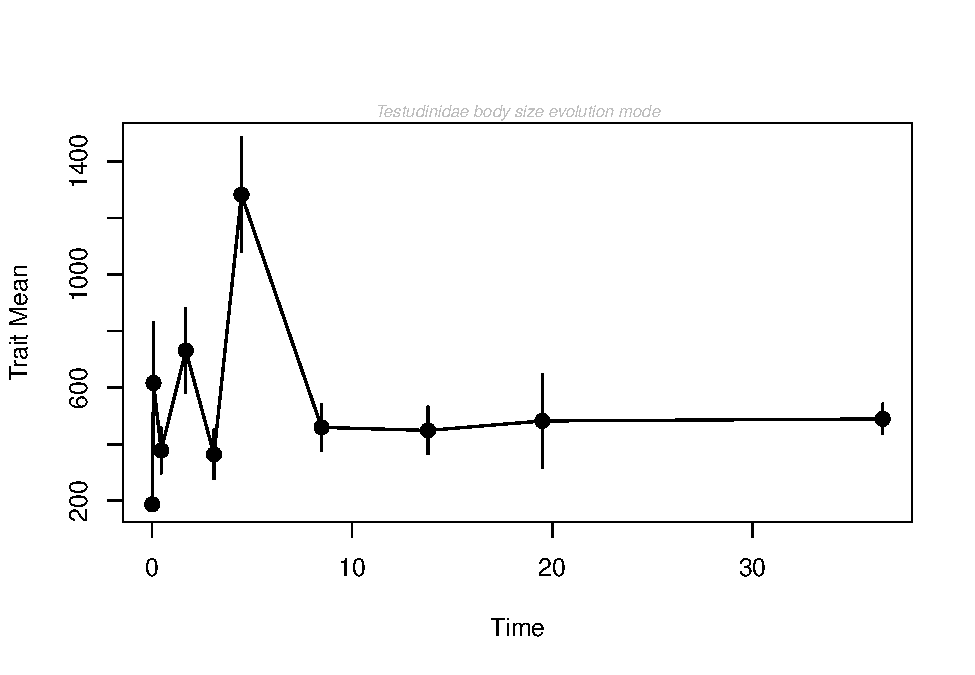
\includegraphics{MA_JJ_files/figure-latex/paleoTS, individuals, Europe-1.pdf}
\caption{Europe, individuals}
\end{figure}

\begin{longtable}[]{@{}lrrrr@{}}
\caption{Model-fitting results for testudinidae, individuals,
Europe}\tabularnewline
\toprule
& logL & K & AICc & Akaike.wt\tabularnewline
\midrule
\endfirsthead
\toprule
& logL & K & AICc & Akaike.wt\tabularnewline
\midrule
\endhead
GRW & -107.36295 & 2 & 219.8168 & 0.000\tabularnewline
URW & -107.36369 & 1 & 217.0607 & 0.001\tabularnewline
Stasis & -99.36654 & 2 & 203.8240 & 0.998\tabularnewline
\bottomrule
\end{longtable}

\newpage 

\subsubsection{Europe, no bins,
individuals}\label{europe-no-bins-individuals}

\begin{figure}[htbp]
\centering
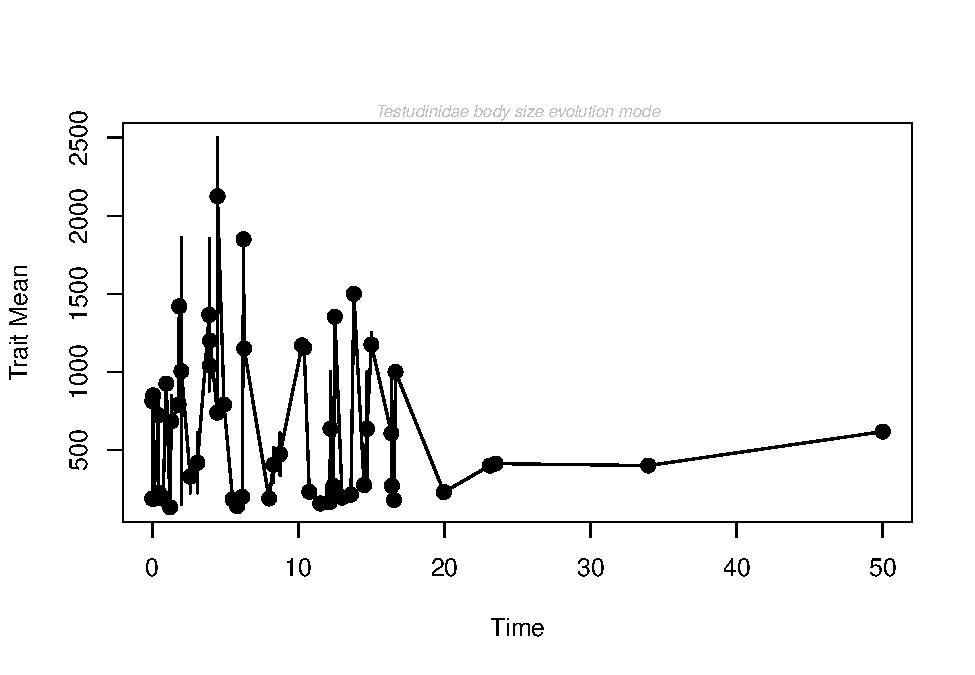
\includegraphics{MA_JJ_files/figure-latex/paleoTS, no bins individuals, Europe-1.pdf}
\caption{Europe, individuals, no bins}
\end{figure}

\begin{longtable}[]{@{}lrrrr@{}}
\caption{Model-fitting results for testudinidae, individuals, no bins,
Europe}\tabularnewline
\toprule
& logL & K & AICc & Akaike.wt\tabularnewline
\midrule
\endfirsthead
\toprule
& logL & K & AICc & Akaike.wt\tabularnewline
\midrule
\endhead
GRW & -447.9212 & 2 & 900.0777 & 0\tabularnewline
URW & -447.9212 & 1 & 897.9194 & 0\tabularnewline
Stasis & -409.6032 & 2 & 823.4417 & 1\tabularnewline
\bottomrule
\end{longtable}

\newpage 

\subsubsection{Europe, no bins, genera}\label{europe-no-bins-genera}

\begin{figure}[htbp]
\centering
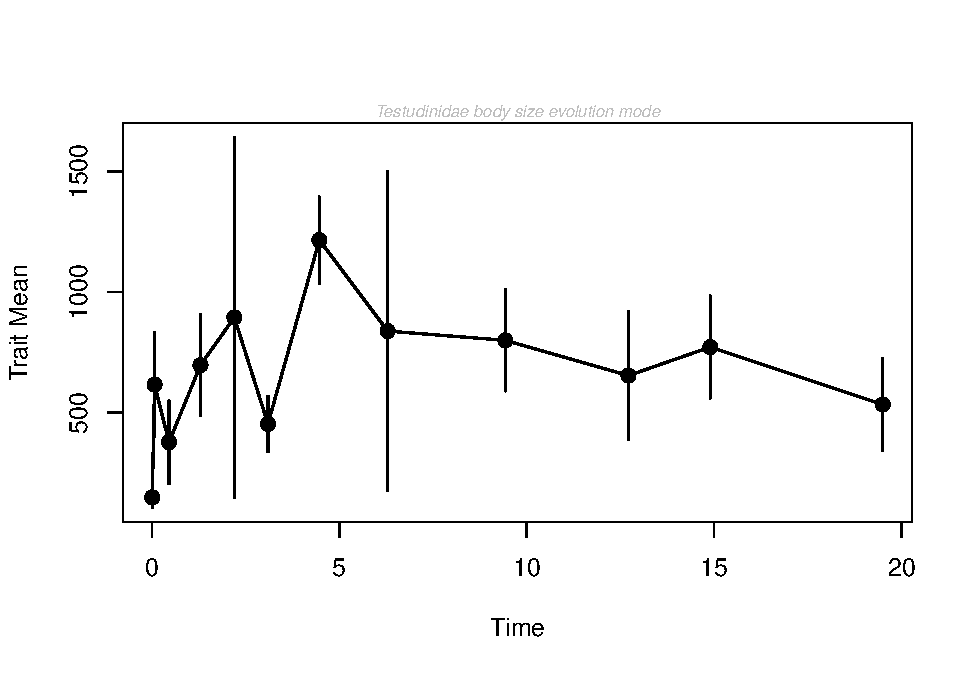
\includegraphics{MA_JJ_files/figure-latex/paleoTS with different time bins, no bins, genera, Europe-1.pdf}
\caption{Mean age of each sample as time bin, genera,Europe}
\end{figure}

\begin{longtable}[]{@{}lrrrr@{}}
\caption{Model-fitting results for testudinidae, no bins,
genera}\tabularnewline
\toprule
& logL & K & AICc & Akaike.wt\tabularnewline
\midrule
\endfirsthead
\toprule
& logL & K & AICc & Akaike.wt\tabularnewline
\midrule
\endhead
GRW & -872.4874 & 2 & 1749.2013 & 0\tabularnewline
URW & -767.6493 & 1 & 1537.3727 & 0\tabularnewline
Stasis & -457.9671 & 2 & 920.1606 & 1\tabularnewline
\bottomrule
\end{longtable}

\newpage

\subsubsection{America, individuals (2nd
try)}\label{america-individuals-2nd-try}

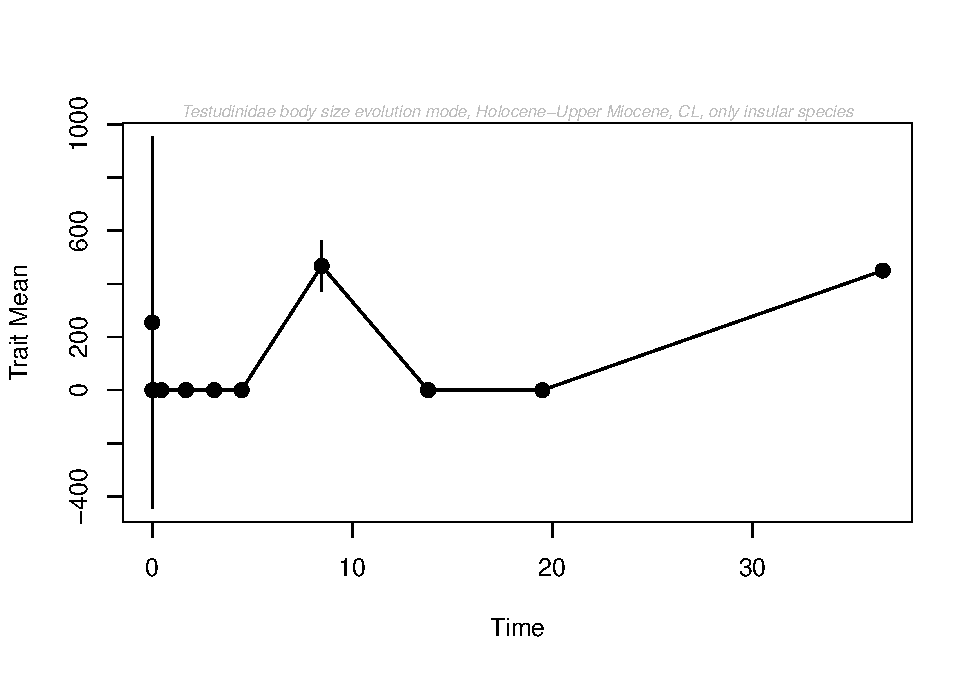
\includegraphics{MA_JJ_files/figure-latex/paleoTS, individuals, America-1.pdf}
fits don't work, no idea why

\newpage

\subsubsection{America, no bins,
individuals}\label{america-no-bins-individuals}

\begin{figure}[htbp]
\centering
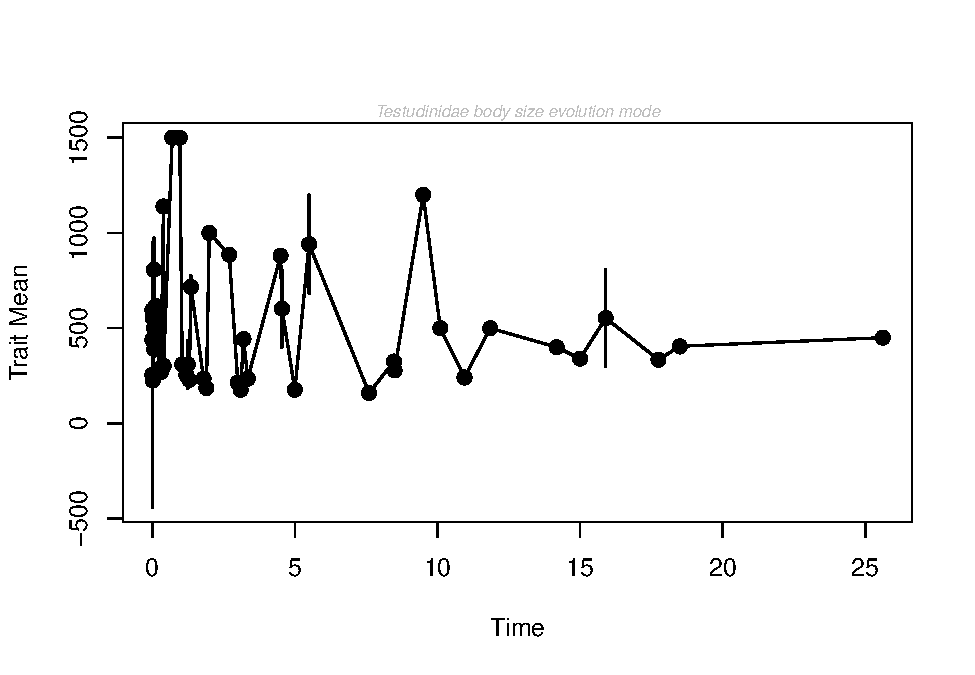
\includegraphics{MA_JJ_files/figure-latex/paleoTS, no bins individuals, America-1.pdf}
\caption{America, individuals, no bins}
\end{figure}

\begin{longtable}[]{@{}lrrrr@{}}
\caption{Model-fitting results for testudinidae, individuals, no bins,
America}\tabularnewline
\toprule
& logL & K & AICc & Akaike.wt\tabularnewline
\midrule
\endfirsthead
\toprule
& logL & K & AICc & Akaike.wt\tabularnewline
\midrule
\endhead
GRW & -849.0212 & 2 & 1702.3215 & 0\tabularnewline
URW & -765.5466 & 1 & 1533.1840 & 0\tabularnewline
Stasis & -334.8158 & 2 & 673.9107 & 1\tabularnewline
\bottomrule
\end{longtable}

\newpage 

\subsubsection{America, no bins, genera}\label{america-no-bins-genera}

\begin{figure}[htbp]
\centering
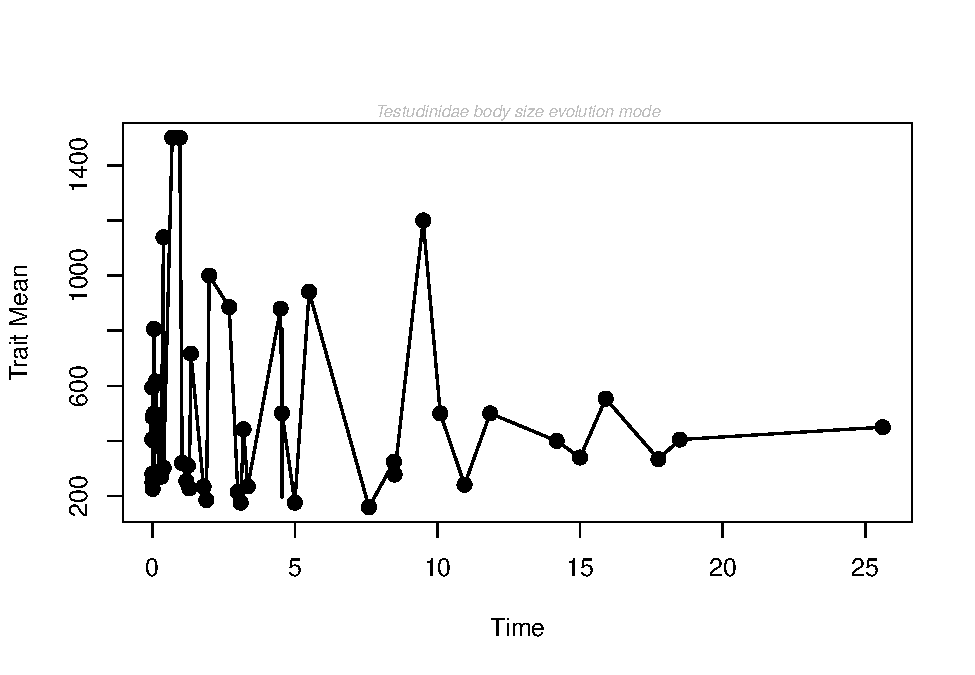
\includegraphics{MA_JJ_files/figure-latex/paleoTS with different time bins, no bins, genera, America-1.pdf}
\caption{Mean age of each sample as time bin, genera, America}
\end{figure}

\begin{longtable}[]{@{}lrrrr@{}}
\caption{Model-fitting results for testudinidae, no bins,
genera}\tabularnewline
\toprule
& logL & K & AICc & Akaike.wt\tabularnewline
\midrule
\endfirsthead
\toprule
& logL & K & AICc & Akaike.wt\tabularnewline
\midrule
\endhead
GRW & -374.4593 & 2 & 753.1977 & 0\tabularnewline
URW & -374.4593 & 1 & 751.0095 & 0\tabularnewline
Stasis & -336.1186 & 2 & 676.5163 & 1\tabularnewline
\bottomrule
\end{longtable}

\newpage

\subsubsection{Asia, individuals}\label{asia-individuals}

\begin{figure}[htbp]
\centering
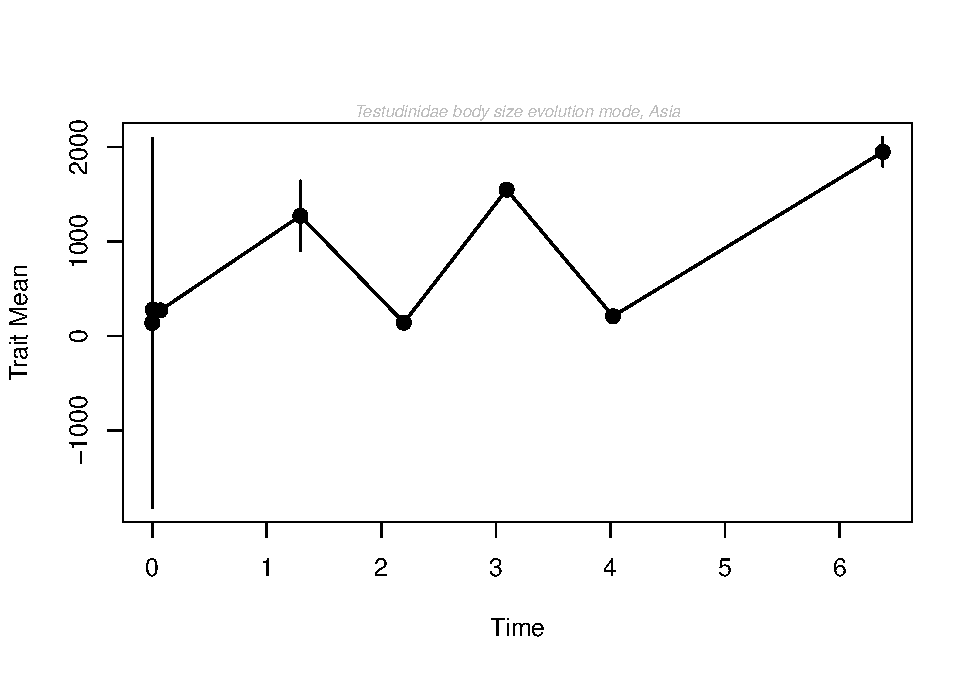
\includegraphics{MA_JJ_files/figure-latex/paleoTS, individuals, Asia-1.pdf}
\caption{individuals, Asia}
\end{figure}

\begin{longtable}[]{@{}lrrrr@{}}
\caption{Model-fitting results for testudinidae, individuals,
Asia}\tabularnewline
\toprule
& logL & K & AICc & Akaike.wt\tabularnewline
\midrule
\endfirsthead
\toprule
& logL & K & AICc & Akaike.wt\tabularnewline
\midrule
\endhead
GRW & -70.79148 & 2 & 148.5830 & 0\tabularnewline
URW & -62.48583 & 1 & 127.7717 & 1\tabularnewline
Stasis & -82.36624 & 2 & 171.7325 & 0\tabularnewline
\bottomrule
\end{longtable}

\newpage

\subsubsection{Asia, no bins,
individuals}\label{asia-no-bins-individuals}

\begin{figure}[htbp]
\centering
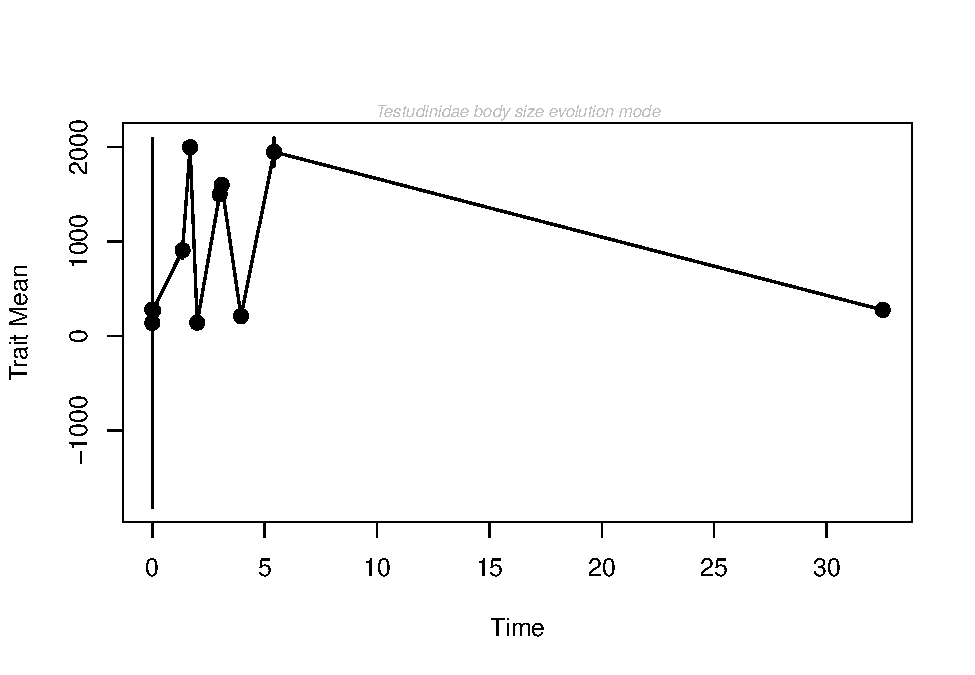
\includegraphics{MA_JJ_files/figure-latex/paleoTS, no bins individuals, Asia-1.pdf}
\caption{Asia, individuals, no bins}
\end{figure}

\begin{longtable}[]{@{}lrrrr@{}}
\caption{Model-fitting results for testudinidae, individuals, no bins,
Asia}\tabularnewline
\toprule
& logL & K & AICc & Akaike.wt\tabularnewline
\midrule
\endfirsthead
\toprule
& logL & K & AICc & Akaike.wt\tabularnewline
\midrule
\endhead
GRW & -131.87801 & 2 & 269.4703 & 0\tabularnewline
URW & -132.23396 & 1 & 266.9679 & 0\tabularnewline
Stasis & -87.44222 & 2 & 180.5987 & 1\tabularnewline
\bottomrule
\end{longtable}

\newpage 

\subsubsection{Asia, no bins, genera}\label{asia-no-bins-genera}

\begin{figure}[htbp]
\centering
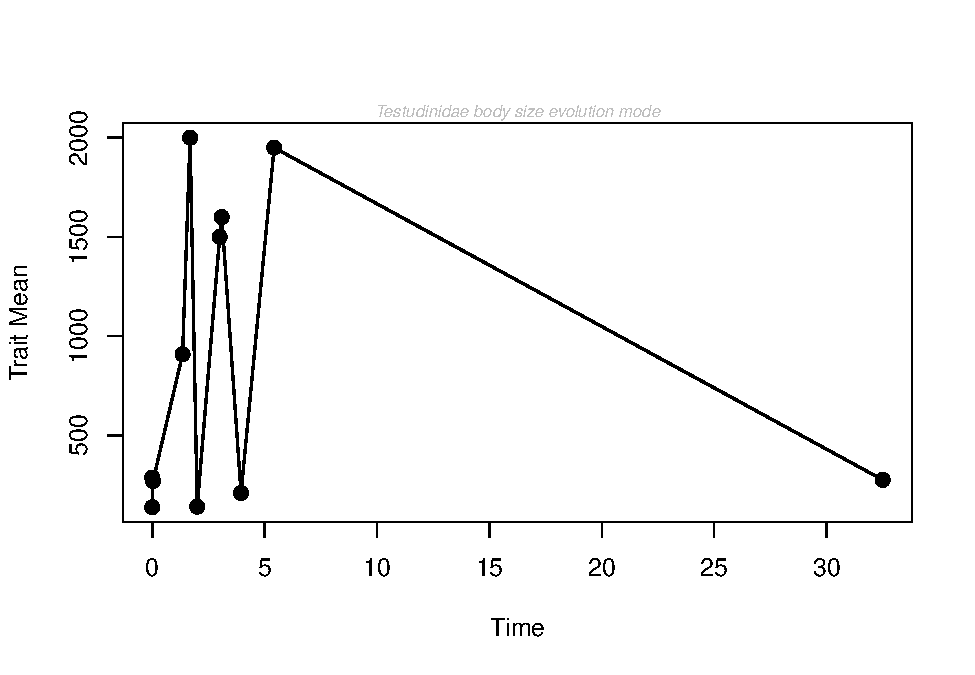
\includegraphics{MA_JJ_files/figure-latex/paleoTS with different time bins, no bins, genera, Asia-1.pdf}
\caption{Mean age of each sample as time bin, genera, Asia}
\end{figure}

\begin{longtable}[]{@{}lrrrr@{}}
\caption{Model-fitting results for testudinidae, no bins,
genera}\tabularnewline
\toprule
& logL & K & AICc & Akaike.wt\tabularnewline
\midrule
\endfirsthead
\toprule
& logL & K & AICc & Akaike.wt\tabularnewline
\midrule
\endhead
GRW & -105.54806 & 2 & 216.8104 & 0\tabularnewline
URW & -105.54484 & 1 & 213.5897 & 0\tabularnewline
Stasis & -80.19133 & 2 & 166.0969 & 1\tabularnewline
\bottomrule
\end{longtable}

\newpage

\subsubsection{Eurasia, individuals}\label{eurasia-individuals}

\begin{figure}[htbp]
\centering
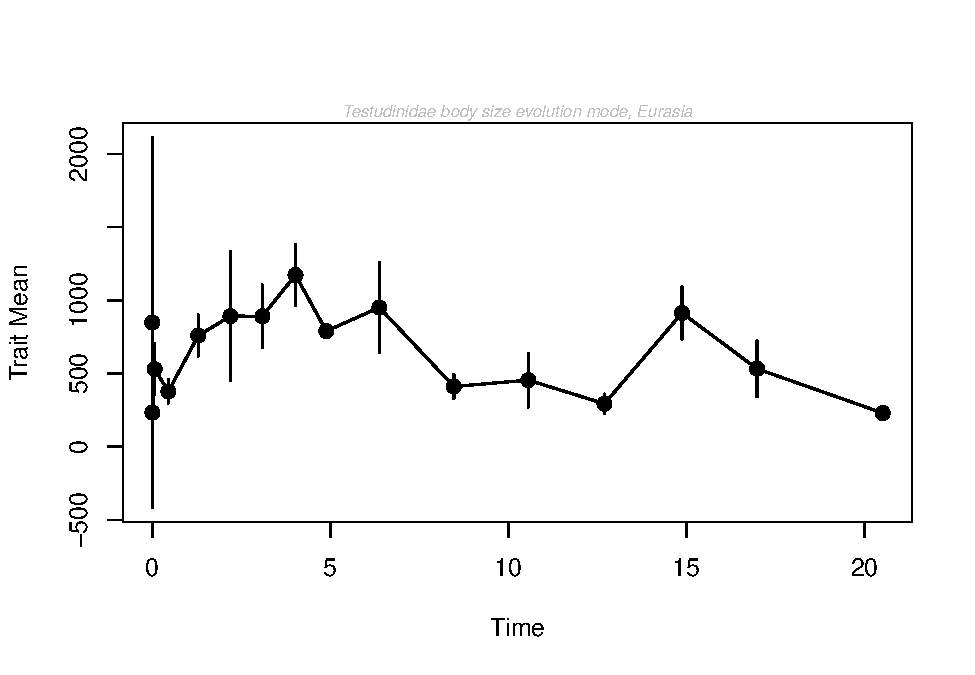
\includegraphics{MA_JJ_files/figure-latex/paleoTS, individuals, Eurasia-1.pdf}
\caption{individuals, Eurasia}
\end{figure}

\begin{longtable}[]{@{}lrrrr@{}}
\caption{Model-fitting results for testudinidae, individuals,
Asia}\tabularnewline
\toprule
& logL & K & AICc & Akaike.wt\tabularnewline
\midrule
\endfirsthead
\toprule
& logL & K & AICc & Akaike.wt\tabularnewline
\midrule
\endhead
GRW & -114.2808 & 2 & 233.5616 & 0.023\tabularnewline
URW & -114.3535 & 1 & 231.0147 & 0.081\tabularnewline
Stasis & -110.6028 & 2 & 226.2055 & 0.896\tabularnewline
\bottomrule
\end{longtable}

\newpage

\subsubsection{Eurasia, no bins,
individuals}\label{eurasia-no-bins-individuals}

\begin{figure}[htbp]
\centering
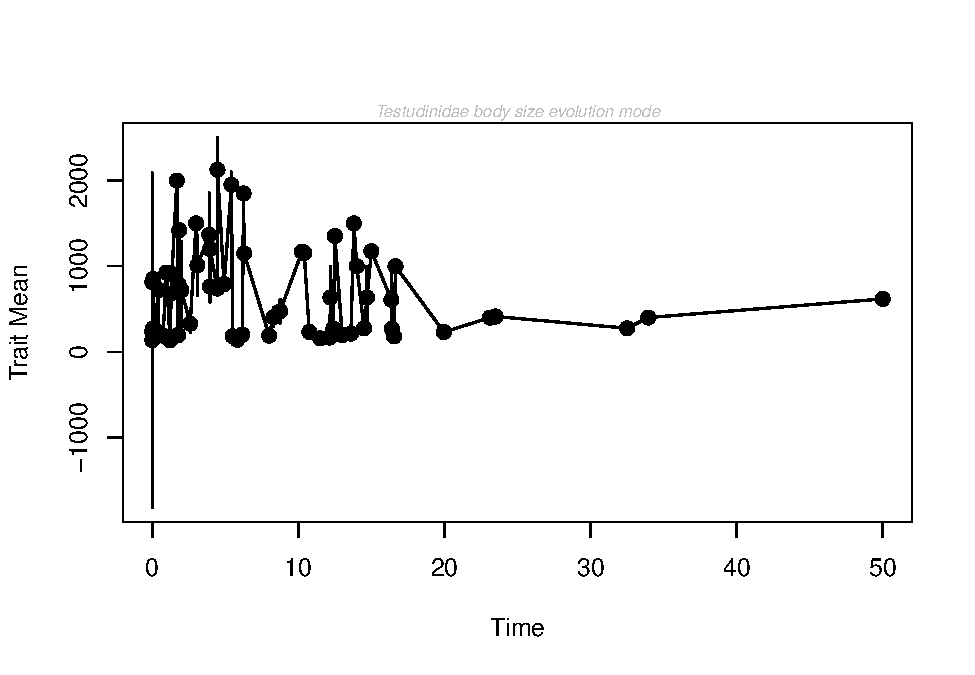
\includegraphics{MA_JJ_files/figure-latex/paleoTS, no bins individuals, Eurasia-1.pdf}
\caption{Eurasia, individuals, no bins}
\end{figure}

\begin{longtable}[]{@{}lrrrr@{}}
\caption{Model-fitting results for testudinidae, individuals, no bins,
Eurasia}\tabularnewline
\toprule
& logL & K & AICc & Akaike.wt\tabularnewline
\midrule
\endfirsthead
\toprule
& logL & K & AICc & Akaike.wt\tabularnewline
\midrule
\endhead
GRW & -1254.0121 & 2 & 2512.224 & 0\tabularnewline
URW & -1193.3477 & 1 & 2388.761 & 0\tabularnewline
Stasis & -600.6003 & 2 & 1205.401 & 1\tabularnewline
\bottomrule
\end{longtable}

\newpage 

\subsubsection{Eurasia, no bins, genera}\label{eurasia-no-bins-genera}

\begin{figure}[htbp]
\centering
\includegraphics{MA_JJ_files/figure-latex/paleoTS with different time bins, no bins, genera, Eurasia-1.pdf}
\caption{Mean age of each sample as time bin, genera, Eurasia}
\end{figure}

\begin{longtable}[]{@{}lrrrr@{}}
\caption{Model-fitting results for testudinidae, no bins,
genera}\tabularnewline
\toprule
& logL & K & AICc & Akaike.wt\tabularnewline
\midrule
\endfirsthead
\toprule
& logL & K & AICc & Akaike.wt\tabularnewline
\midrule
\endhead
GRW & -2350.1503 & 2 & 4704.5006 & 0\tabularnewline
URW & -1237.0573 & 1 & 2476.1801 & 0\tabularnewline
Stasis & -484.4122 & 2 & 973.0243 & 1\tabularnewline
\bottomrule
\end{longtable}


\end{document}
